%%%%%%%%%%%%%%%%%%%%%%%%%%%%%%%%
%%  Capítulo 5: Resultados experimentales  %%
%%%%%%%%%%%%%%%%%%%%%%%%%%%%%%%%


%%%%
\section{Construcción del reflector}
\label{sec_resultados_cons_ref}
%%%%

Si bien la construcción del reflector y la medición del alimentador en conjunto con el reflector no es objeto de la presente tesis, el mismo se ha diseñado e implementado durante el cursado de la asignatura \emph{Propagación y sistemas irradiantes}.
%%%%
\begin{figure} [H]
\centering 
\subfigure[Vista anterior.]{
\label{fig_resultados:1}
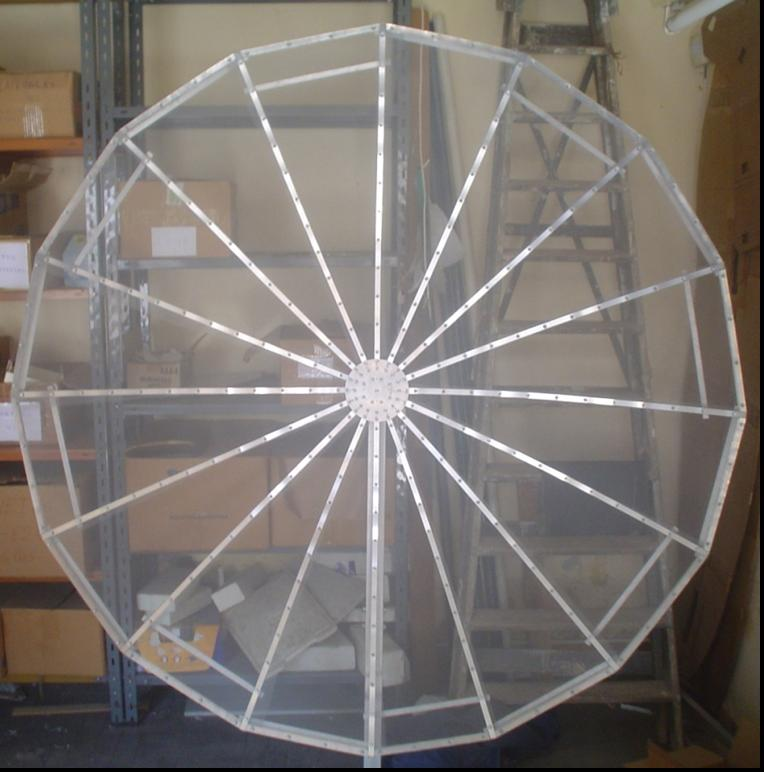
\includegraphics[scale = 0.4]{Figures/Resultados/resultados_1}}
\hspace{5mm}
\subfigure[Vista lateral.]{
\label{fig_resultados:2}
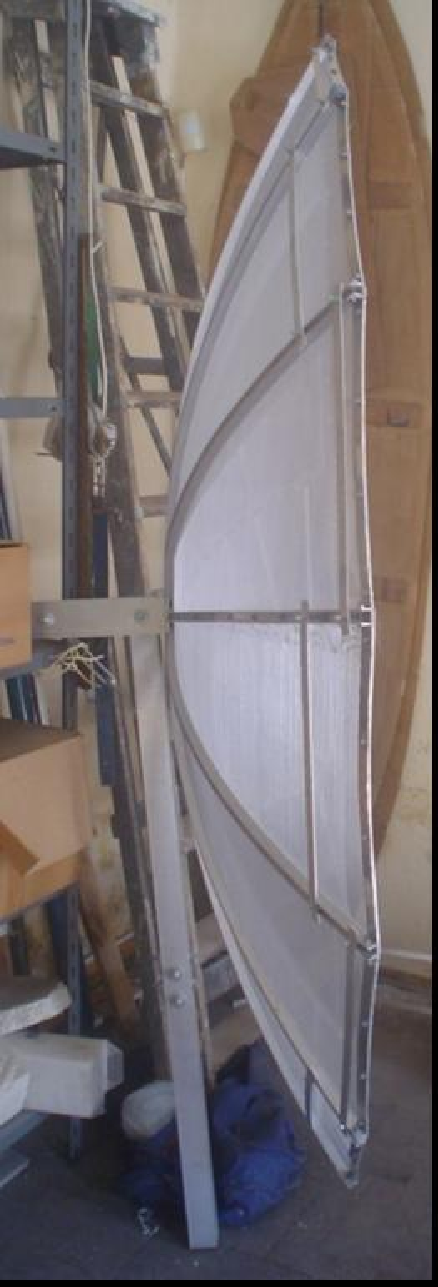
\includegraphics[scale = 0.4]{Figures/Resultados/resultados_2}}
\caption{Reflector parabólico implementado.}
\label{grup_fig_resultados:1}
\end{figure}
%%%%
En las secciones \ref{sec_resultados_sim_pol_cru} y \ref{sec_resultados_sim_dia_rad} se muestran las simulaciones del conjunto formado por el alimentador con el reflector parabólico.

%%%%
\section{Construcción del alimentador}
\label{sec_resultados_cons_alim}
%%%%

La primer duda surgida al momento de comenzar la construcción del alimentador fue determinar con que material se construiría. Se analizaron 4 tipos de materiales conductores: dos metales puros, aluminio y cobre, y dos aleaciones, bronce y latón. Las características generales de cada material son:
%%%%
\begin{itemize}
\item Aluminio: Posee elevada conductividad, baja densidad, precio relativamente bajo y existe una gran cantidad de medidas de caños normalizados. Presenta el inconveniente de que no es posible unir las distintas partes del alilmentador con un soldador de estaño, por lo que es necesario utilizar una soldadora de arco.
\item Cobre: Posee mayor conductividad y densidad que el aluminio, y las distintas partes del alimentador pueden unirse con un soldador de estaño. Como desventaja, es un material costoso y frecuenctemente no se consigue en las medidas estandarizadas.
\item Bronce: Es una aleación de cobre y estaño y su conductividad, si bien es menor que la del cobre y del aluminio, depende del porcentaje de cobre y de estaño que tenga la aleación. De densidad similar a la del cobre, se encuentra disponible en una gran variedad de medidas estandarizadas, y su precio es menor que el del cobre. Al igual que el cobre, pueden unirse las distintas partes del alimentador con un soldador de estaño.
\item Latón: Es una aleación de cobre y zinc, y presenta características similares al bronce, aunque sus propiedades dependen del porcentaje de cobre y de zinc. Al igual que el bronce, se encuentra disponible en una amplia variedad de medidas normalizadas, y es soldable con estaño.
\end{itemize}
%%%%
Por las características eléctricas y su disponibilidad, se empleó latón para la implementación del alimentador. Para la construcción de la guía de onda cilíndrica, se utilizó un caño de sección circular con las siguientes características \cite{laton}:
%%%%
\begin{itemize}
\item Tipo de aleación: Cobre 70 \% - Zinc 30 \%
\item Conductividad: 16,24 $\prodvec$ 10$^{6}$ S/m
\item Diámetro externo: 82,6 mm
\item Espesor: 3 mm
\item Longitud: 255 mm
\end{itemize}
%%%%
El caño de latón fue torneado para que su diámetro interior sea de 79,2 mm y, posteriormente, se le realizó un agujero que es donde se colocó el conector N para alimentar la antena, a una distancia de 163,7 mm (calculada en la sección \ref{sec_estudio_dimen}) de la abertura.
%%%%
\begin{figure}[H]
\centering
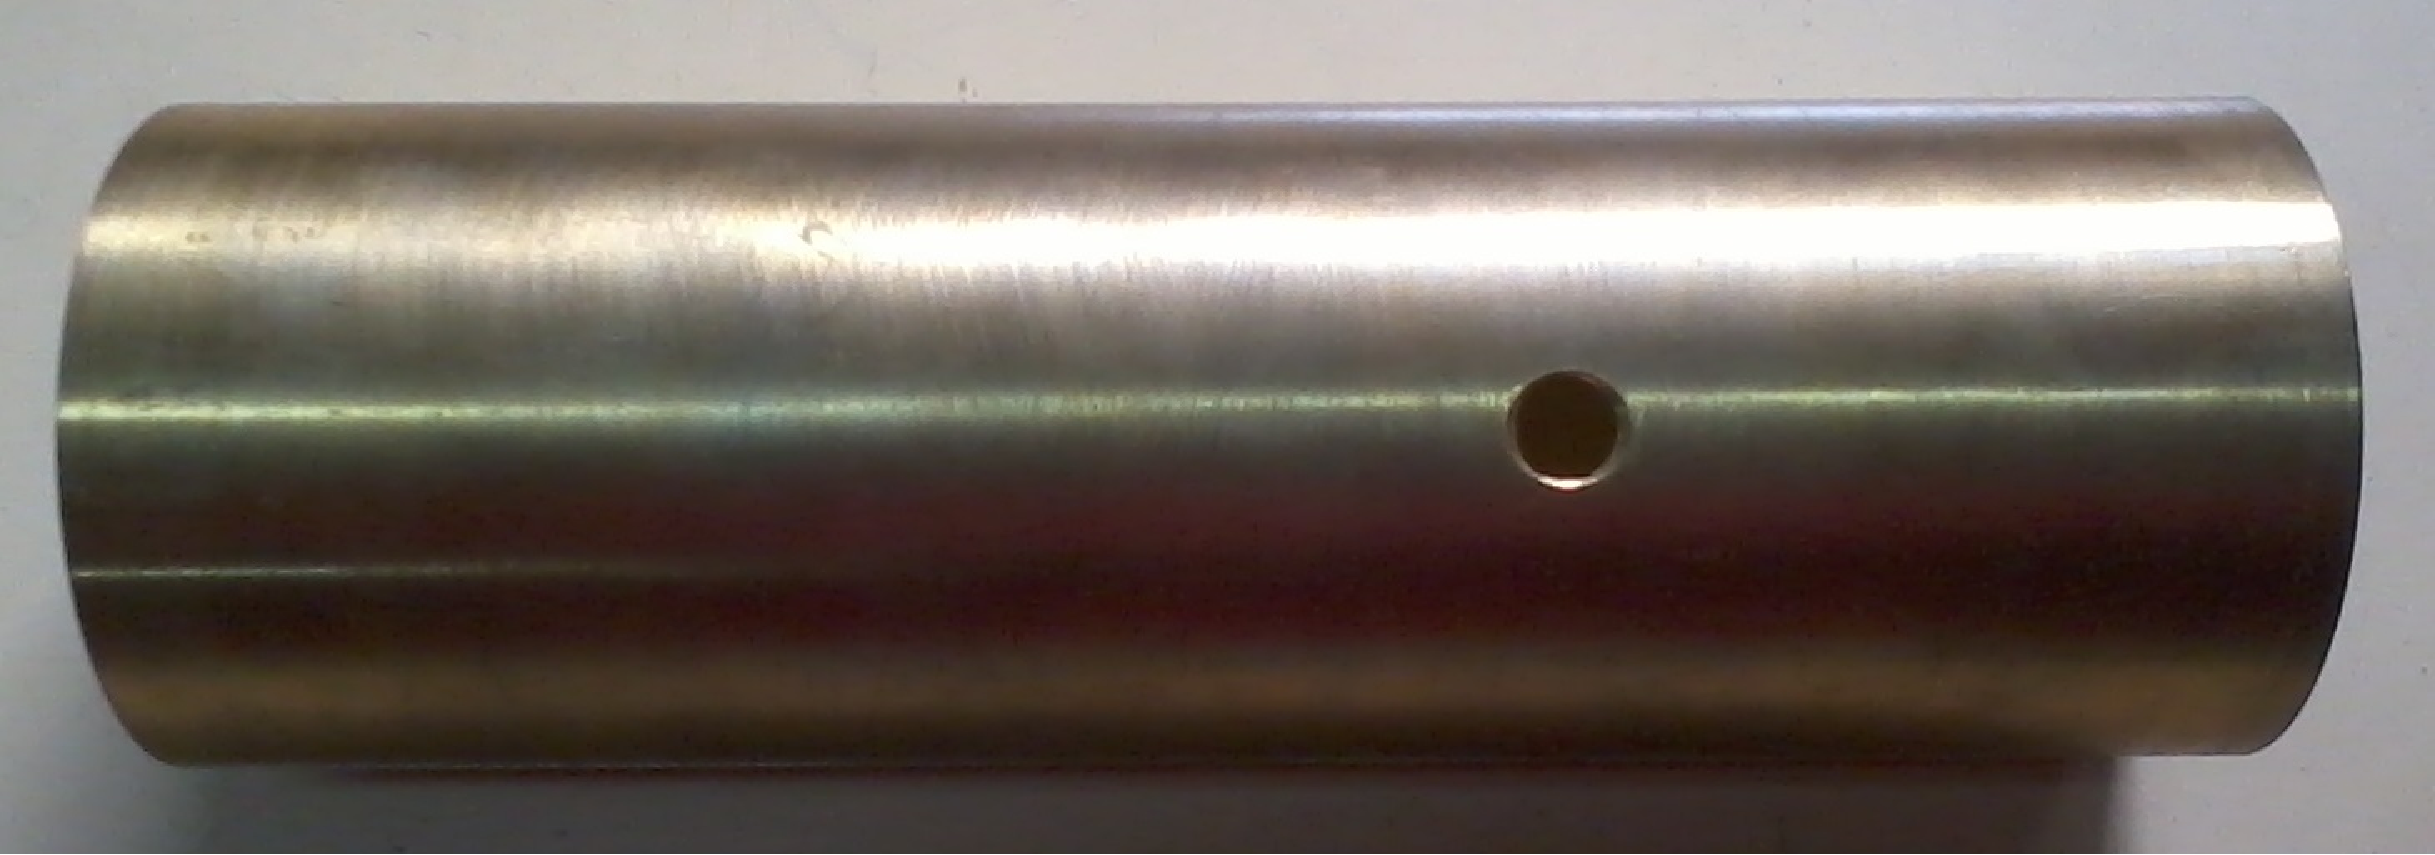
\includegraphics[scale = 0.25]{Figures/Resultados/resultados_3}
\caption{Guía de onda cilíndrica torneada y agujereada.}
\label{fig_resultados:3}
\end{figure}
%%%%
Dado que se utiliza un conector N con montaje a chasis, para el correcto montaje del conector sobre la pared de la guía cilíndrica se soldó una chapa de las mismas dimensiones del conector para que éste disponga de una superficie plana donde colocarse.
%%%%
\begin{figure} [H]
\centering 
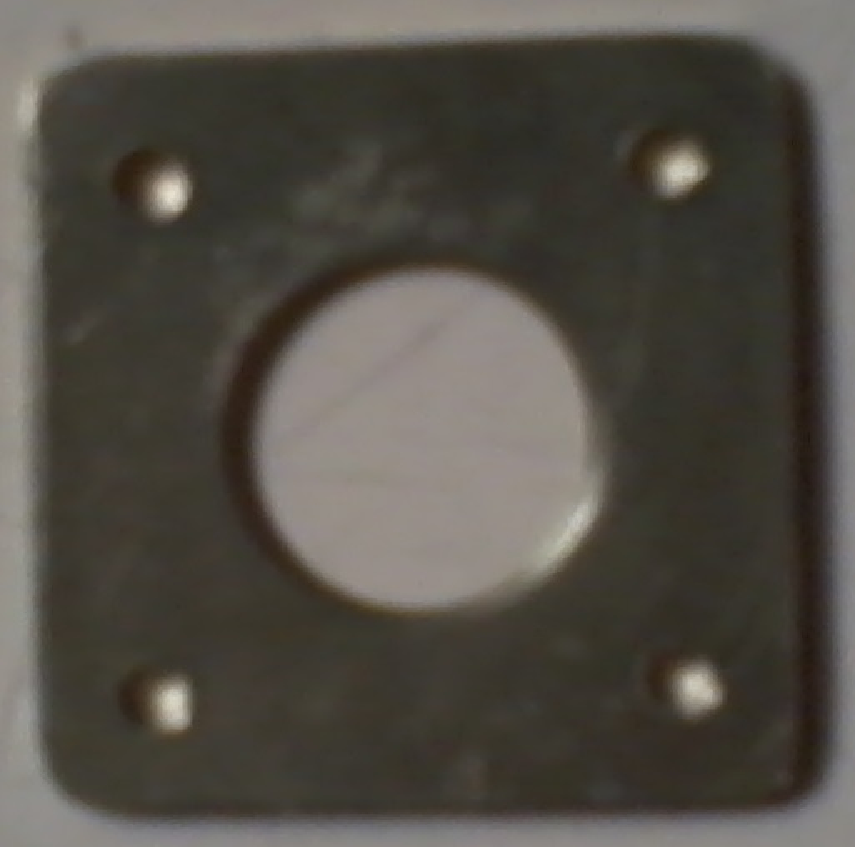
\includegraphics[scale = 0.2]{Figures/Resultados/resultados_4}
\caption{Chapa de montaje del conector N.}
\label{fig_resultados:4}
\end{figure}
%%%%
%%%%
\begin{figure} [H]
\centering 
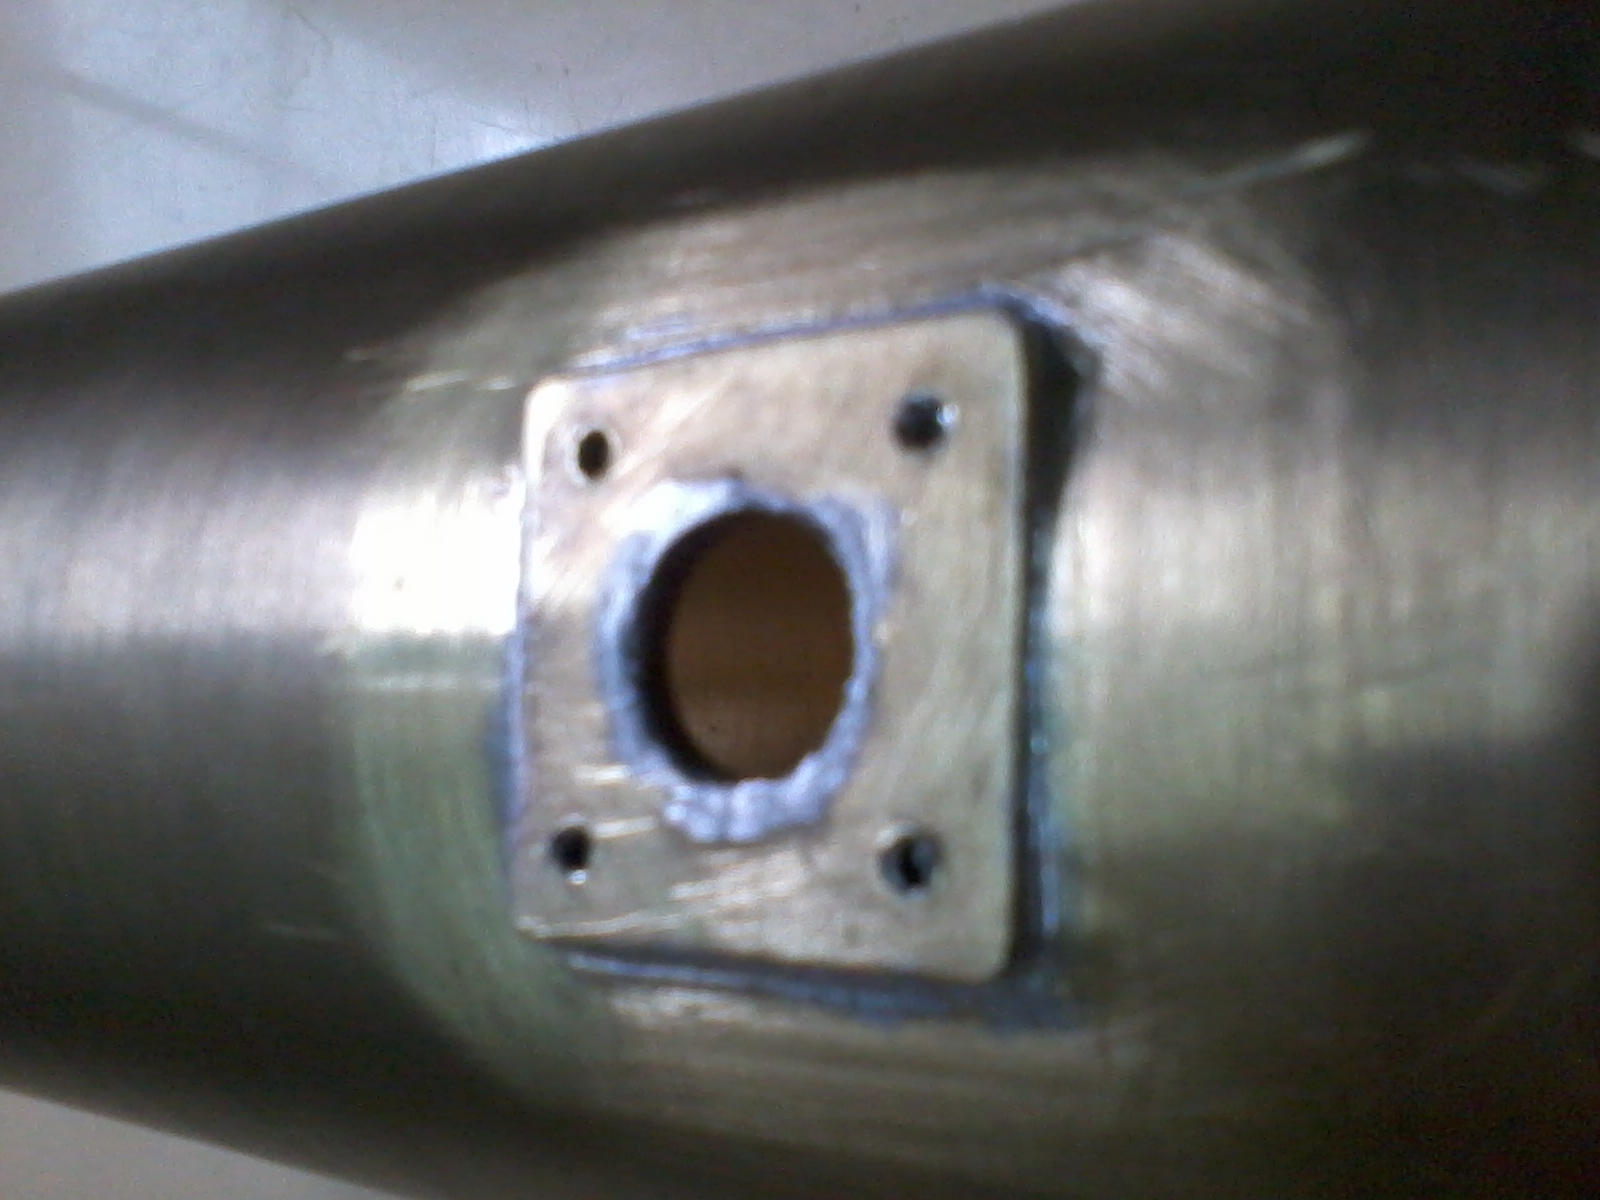
\includegraphics[scale = 0.17]{Figures/Resultados/resultados_5}
\caption{Chapa de montaje soldada a la guía de onda.}
\label{fig_resultados:5}
\end{figure}
%%%%
Para el armado del choque, se utilizó un molde de madera con una abrazadera de acero para curvar una chapa de bronce y darle la forma anular. Una vez que se obtuvo la estructura en forma de anillo, se soldó a una corona circular, cuyo diámetro interno se corresponde con el diámetro externo de la guía de onda.
%%%%
\begin{figure} [H]
\centering 
\subfigure[Vista inferior.]{
\label{fig_resultados:6}
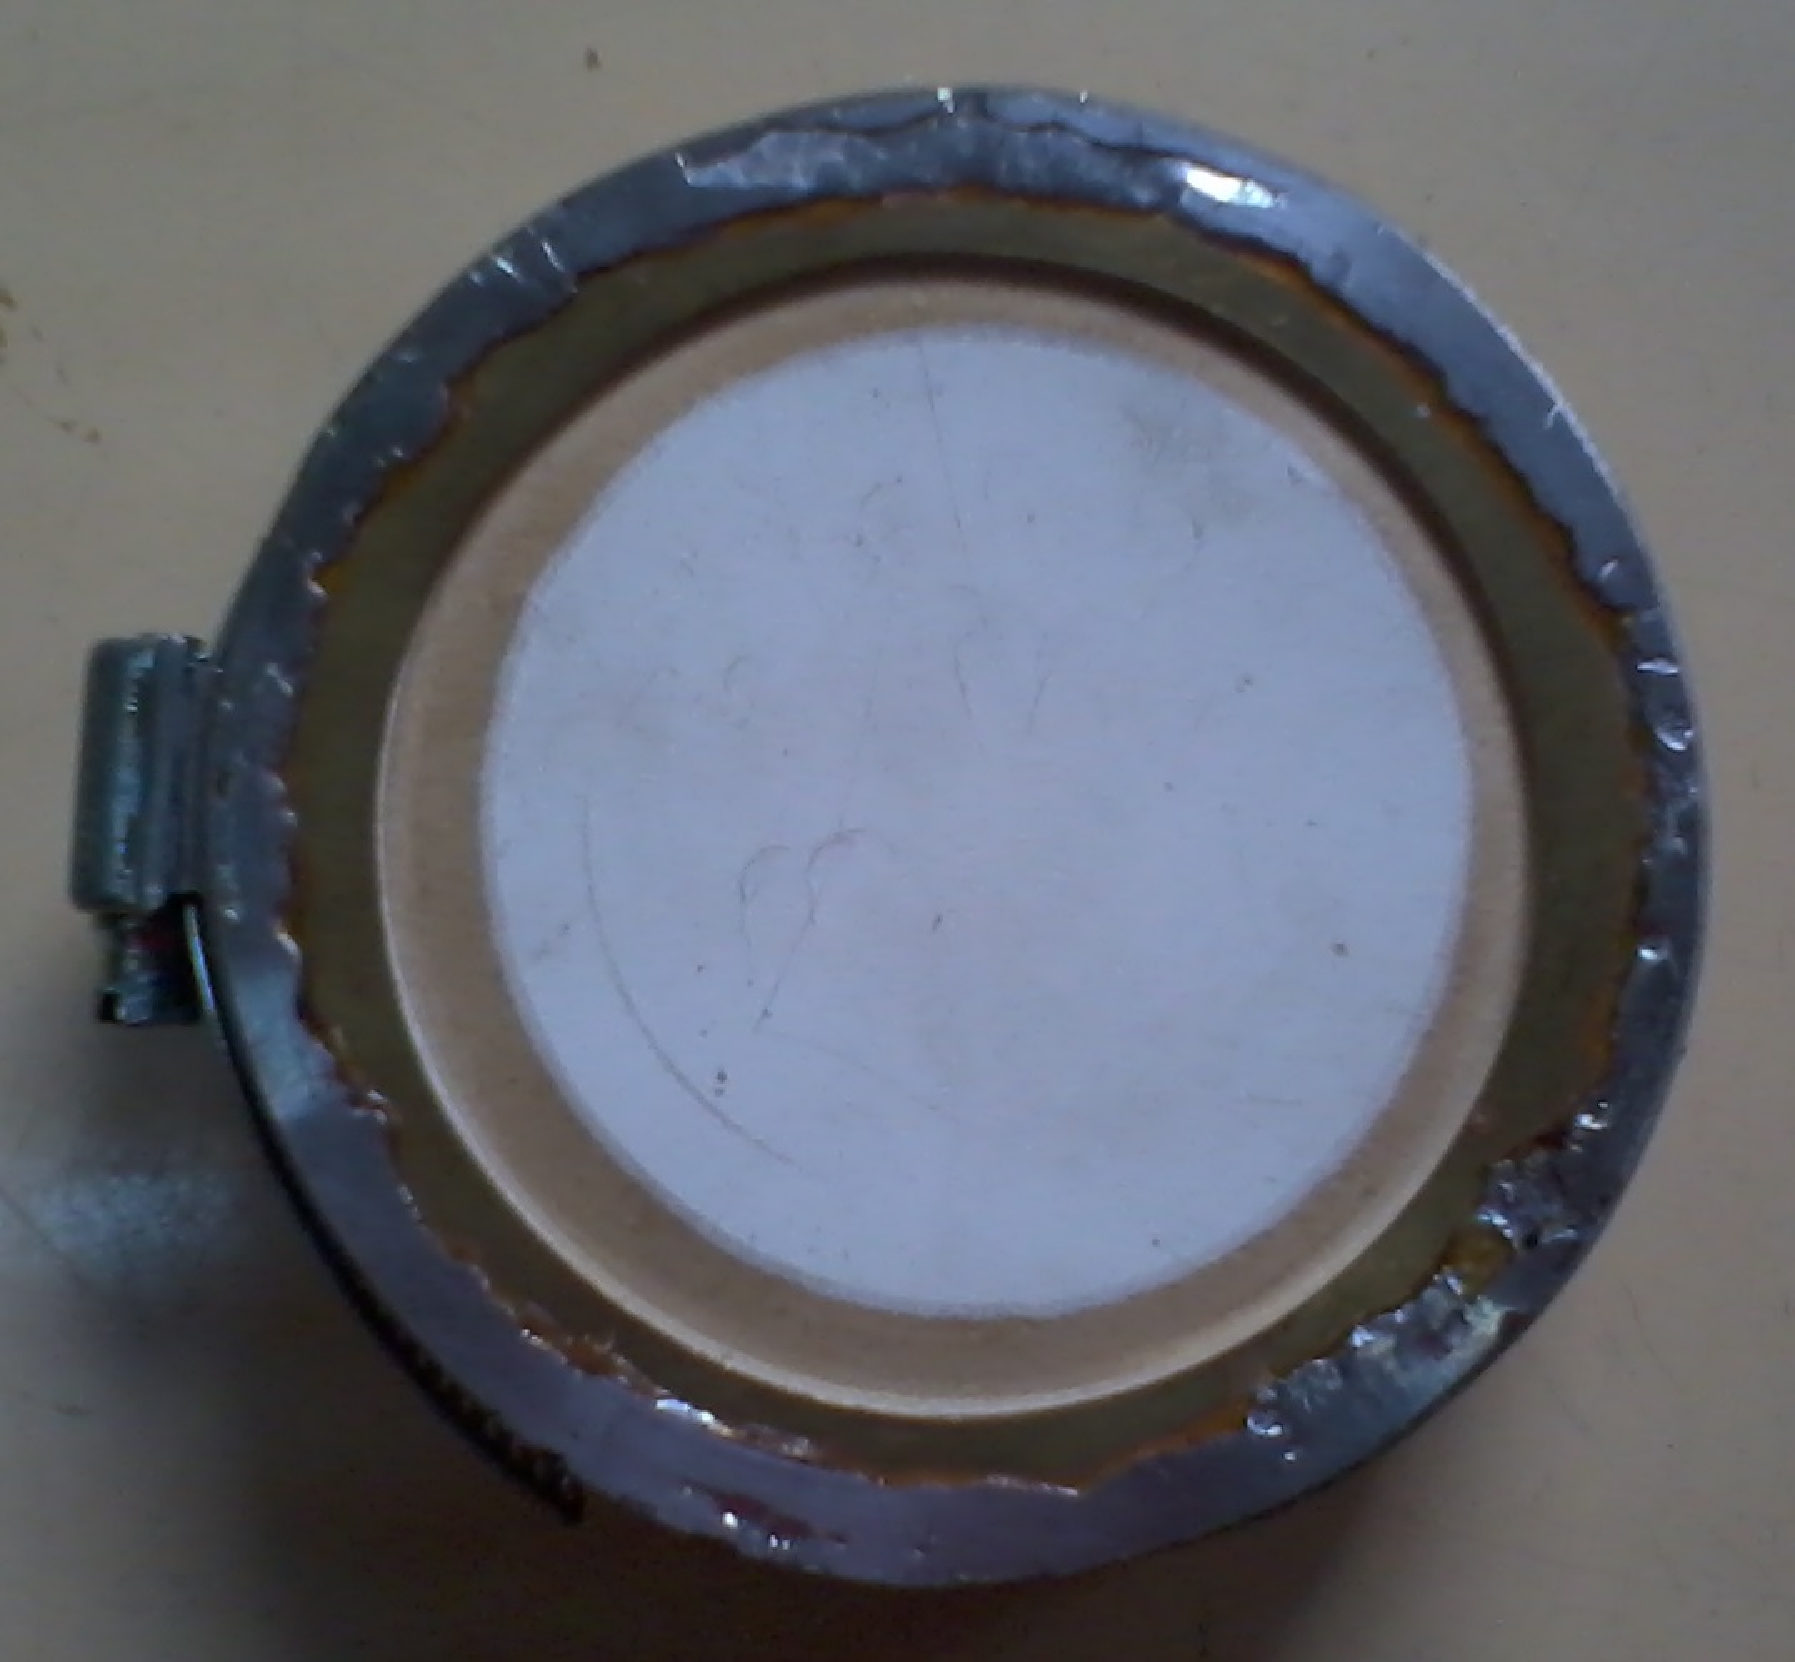
\includegraphics[scale = 0.27]{Figures/Resultados/resultados_6}}
\hspace{5mm}
\subfigure[Vista lateral.]{
\label{fig_resultados:7}
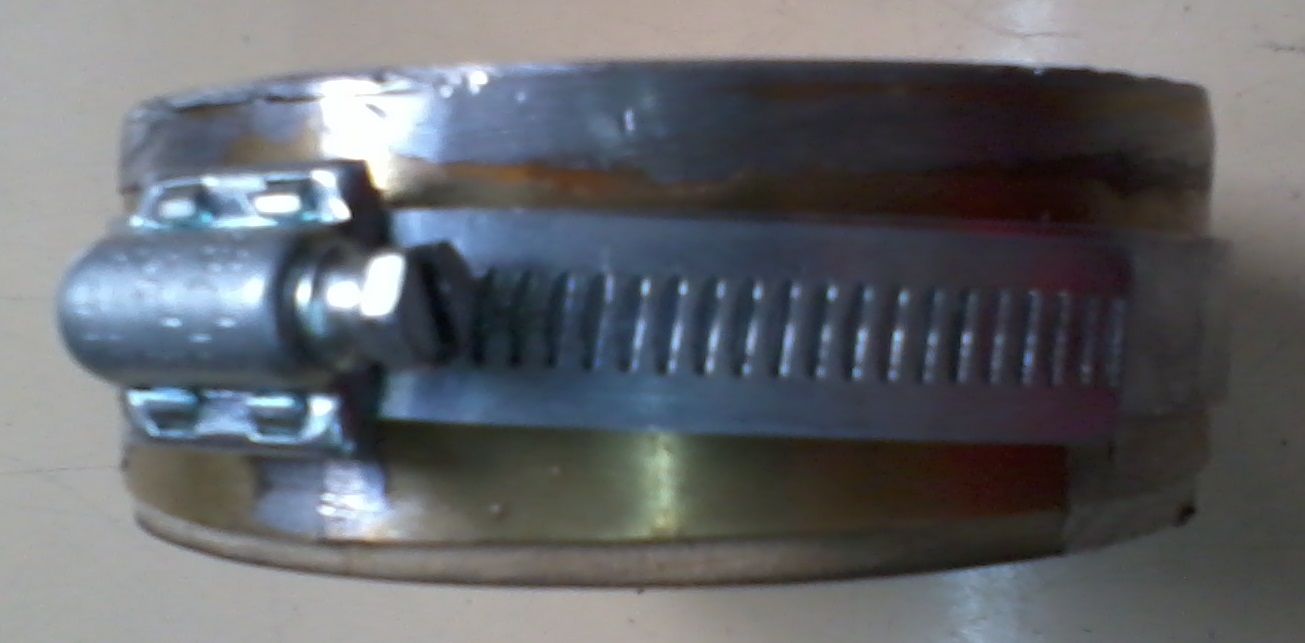
\includegraphics[scale = 0.27]{Figures/Resultados/resultados_7}}
\caption{Choque armado y soldado a partir de un molde de madera.}
\label{grup_fig_resultados:2}
\end{figure}
%%%%
Para excitar la guía de onda, se utilizó un conductor cilíndrico de cobre de diámetro 4,1 mm y de longitud 31,2 mm, que fue soldado al conector N.
%%%%
\begin{figure} [H]
\centering 
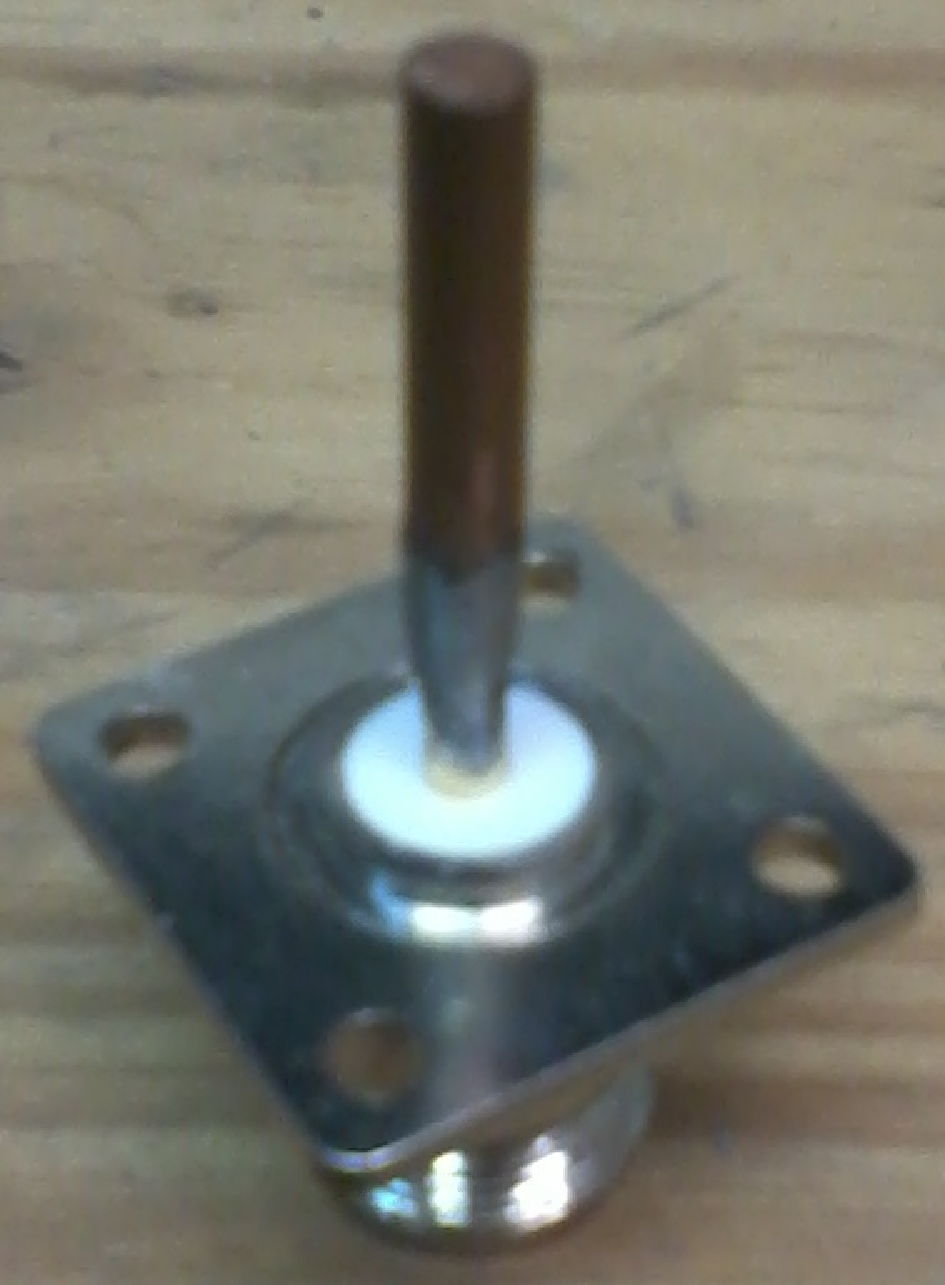
\includegraphics[scale = 0.25]{Figures/Resultados/resultados_8}
\caption{Excitador soldado al conector N.}
\label{fig_resultados:8}
\end{figure}
%%%%
Finalmente, se montó el excitador al alimentador y se soldó el choque, como se observa en la figura \ref{fig_resultados:9}.
%%%%
\begin{figure} [H]
\centering 
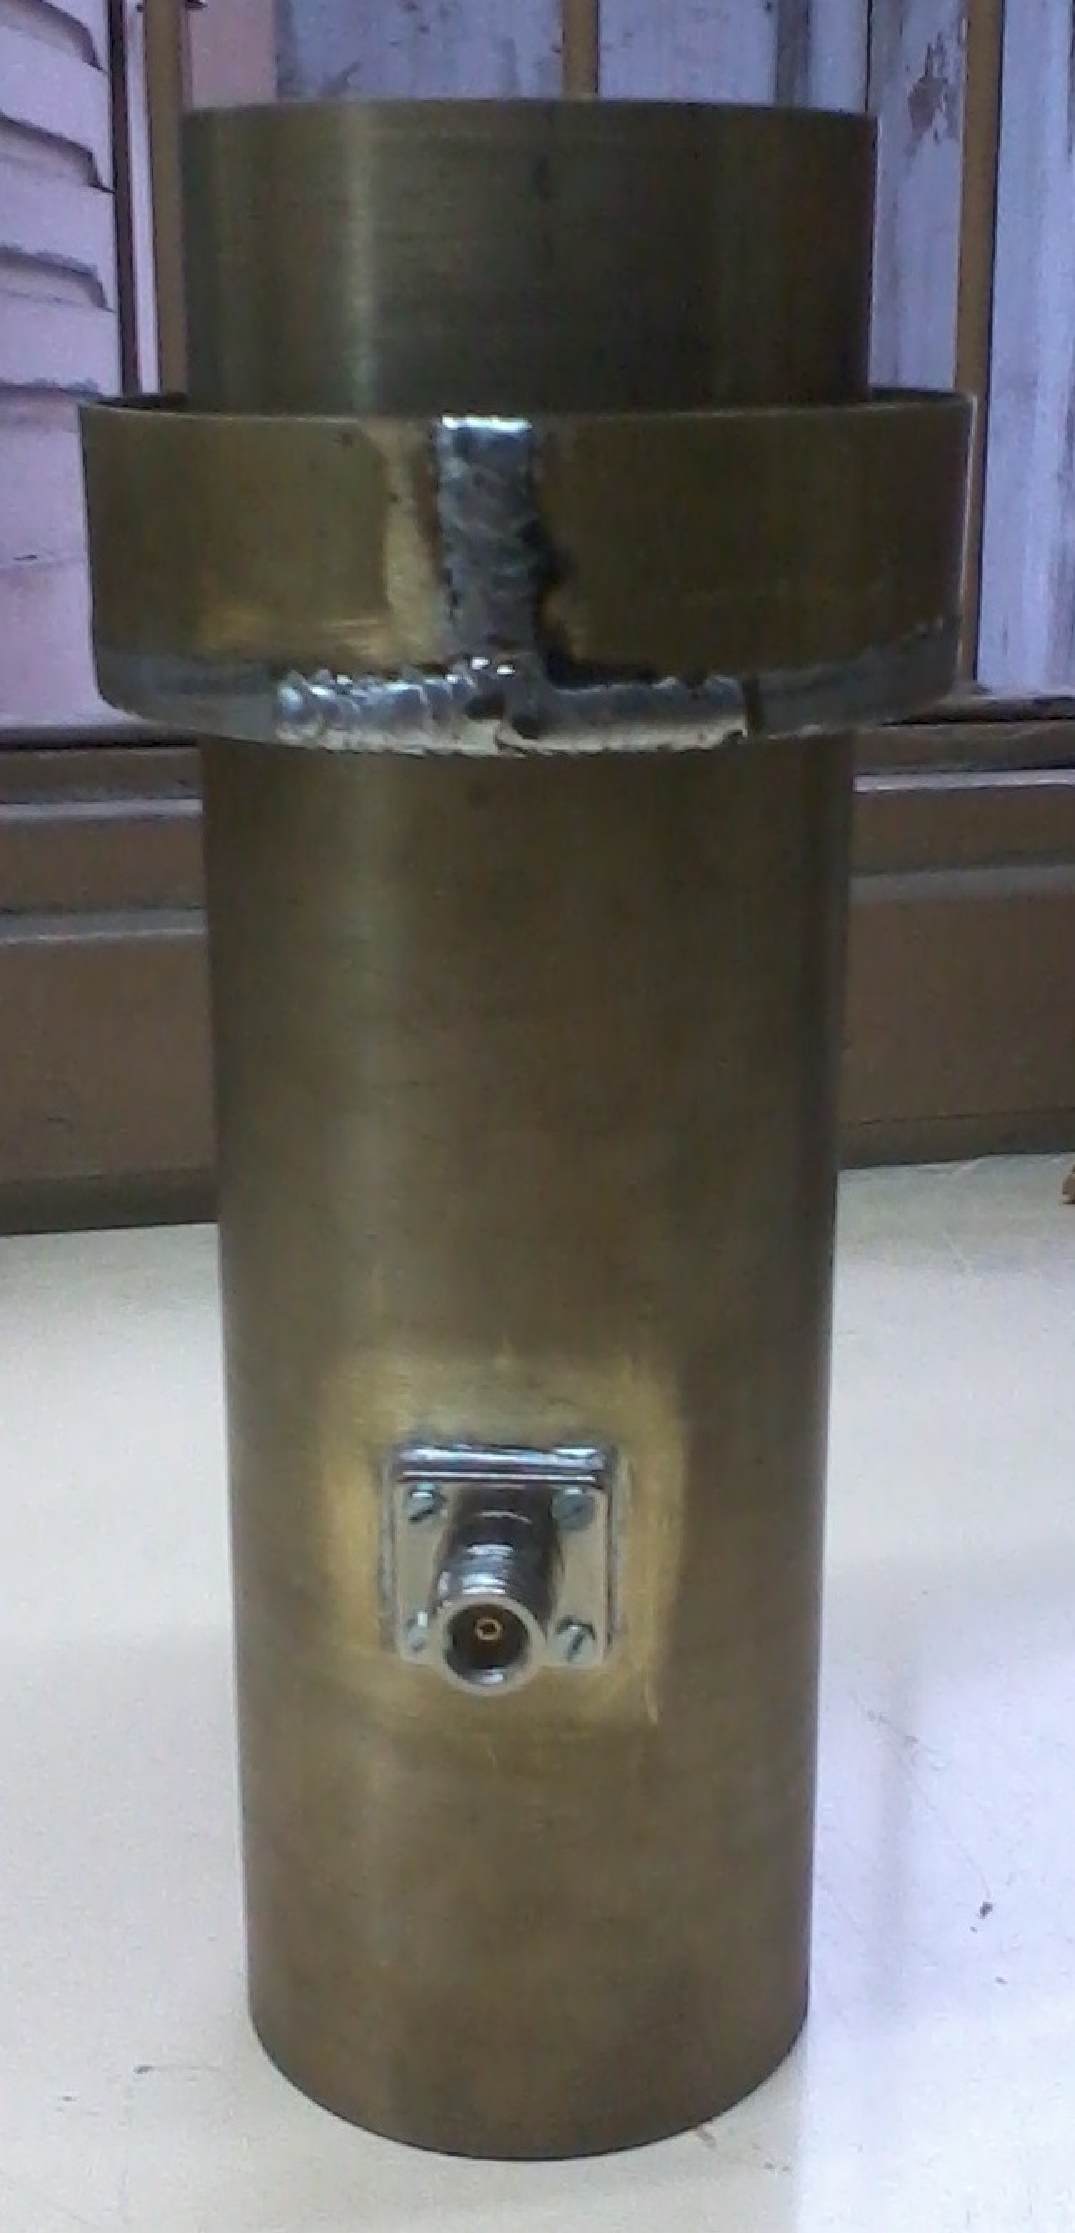
\includegraphics[scale = 0.25]{Figures/Resultados/resultados_9}
\caption{Alimentador con el choque soldado y el conector N.}
\label{fig_resultados:9}
\end{figure}
%%%%
En la próxima sección se explica como se ha determinado experimentalmente la distancia entre el excitador y el corto de la guía de onda y la longitud del excitador.

%%%%
\section{Medición de la impedancia y de la ROE}
\label{sec_resultados_med_imp_roe}
%%%%

Para medir la impedancia y la ROE del alimentador, se implementó el banco de medición de la figura \ref{fig_resultados:10}.
%%%%
\begin{figure} [H]
\centering 
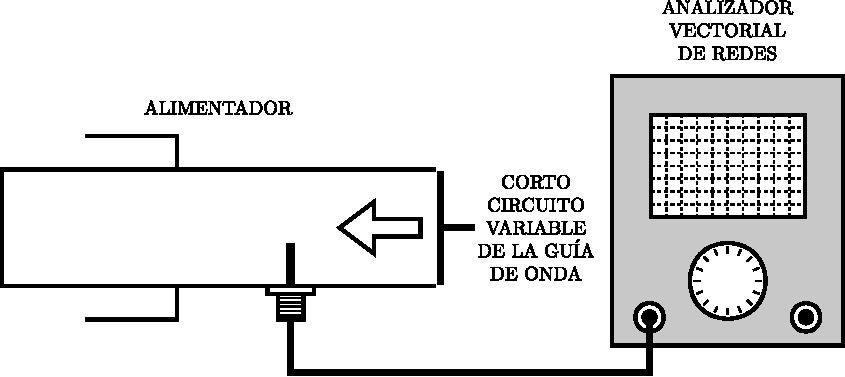
\includegraphics[scale = 1]{Figures/Resultados/resultados_10}
\caption{Banco de medición de la ROE y de la impedancia del alimentador.}
\label{fig_resultados:10}
\end{figure}
%%%%
%%%%
\begin{figure} [H]
\centering 
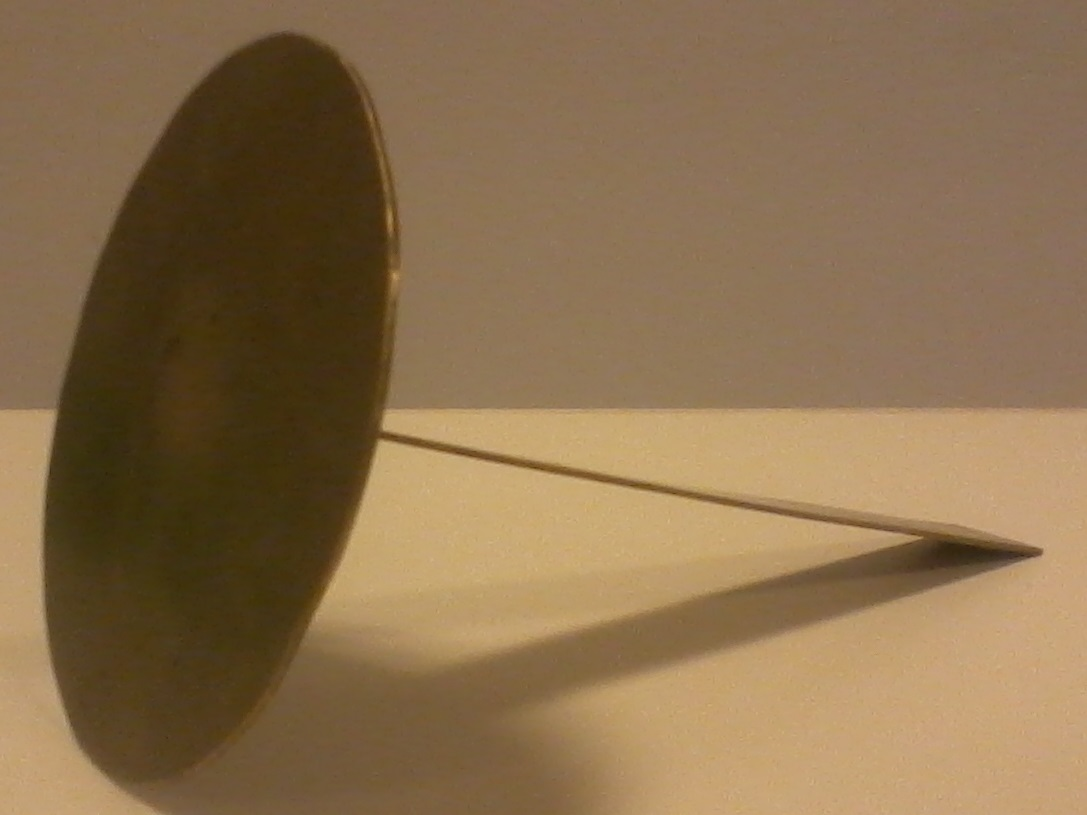
\includegraphics[scale = 0.3]{Figures/Resultados/resultados_11}
\caption{Cortocircuito variable de la guía de onda.}
\label{fig_resultados:11}
\end{figure}
%%%%
El cortocircuito variable de la guía de onda consiste en un círculo de latón que se va desplazando por el interior de la guía; de esta forma se logra variar la distancia entre el cortocircuito y el excitador, y así se puede minimizar la ROE del alimentador y observar la variación en el VNA. Para asegurarse de que haya buen contacto eléctrico entre la tapa que hace de cortocircuito y la guía de onda, se aplicó grasa conductora de cobre a la pared interior de la guía de onda. También se ajustó la longitud del excitador para minimizar la ROE.
%%%%
\begin{figure}[H]
\centering
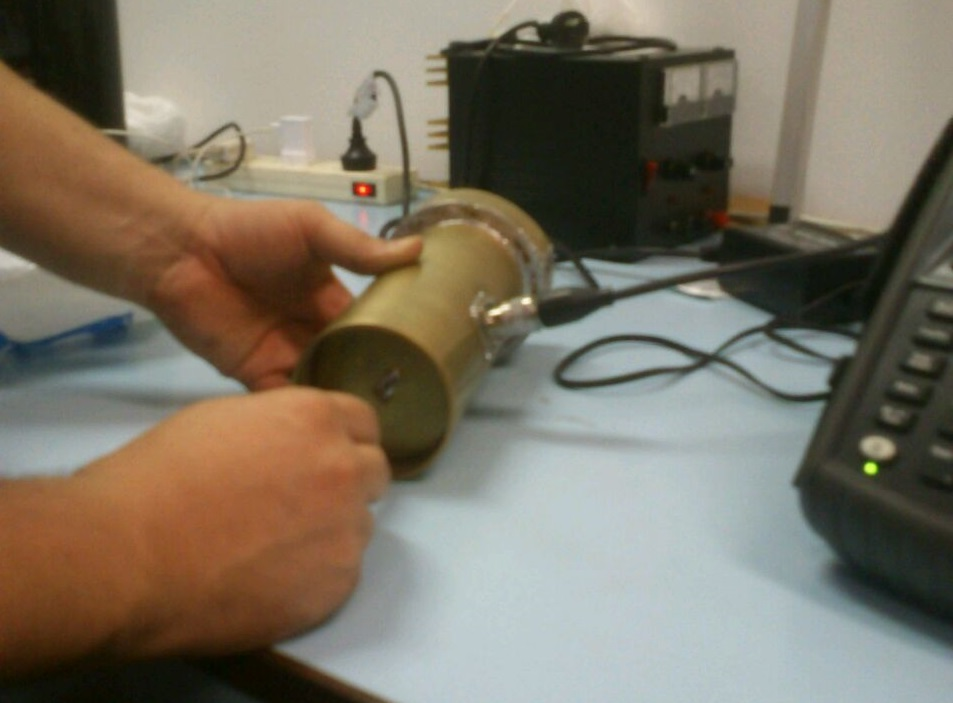
\includegraphics[scale = 0.4]{Figures/Resultados/resultados_12}
\caption{Medición de la ROE y de la impedancia del alimentador.}
\label{fig_resultados:12}
\end{figure}
%%%%
En la tabla \ref{tabla_mediciones:1} se comparan las dimensiones del alimentador determinadas por la simulación y la medición.
%%%%
\begin{table}[H]
\centering
\begin{tabular}{|c|c|c|c|}
\hline
Dimensiones & $L_e$ (mm) & $D_c$ (mm) & Longitud del alimentador (mm)\\
\hline
Simulación & 29,2 & 42,3 & 206,0\\
\hline
Medición & 29,1 & 46,3 & 210,0\\
\hline
\end{tabular}
\caption{Comparación entre las dimensiones del alimentador y del excitador determinadas por simulación y medición.}
\label{tabla_mediciones:1}
\end{table}
%%%%
Se muestran a continuación los gráficos de la impedancia y de la ROE medidas, en las figuras \ref{fig_resultados:13}, \ref{fig_resultados:14} y \ref{fig_resultados:15}, para las dimensiones óptimas determinadas experimentalmente, y se comparan con las simulaciones a fin de contrastar los resultados.
%%%%
\begin{figure}[H]
\centering
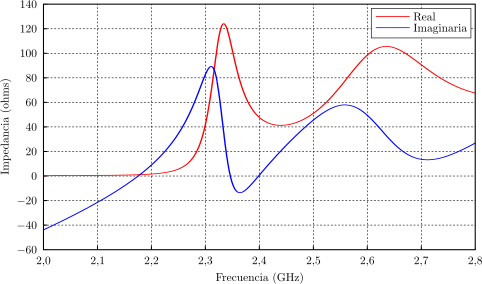
\includegraphics[scale = 1]{Figures/Resultados/resultados_13}
\caption{Simulación de la impedancia del alimentador.}
\label{fig_resultados:13}
\end{figure}
%%%%
%%%%
\begin{figure}[H]
\centering
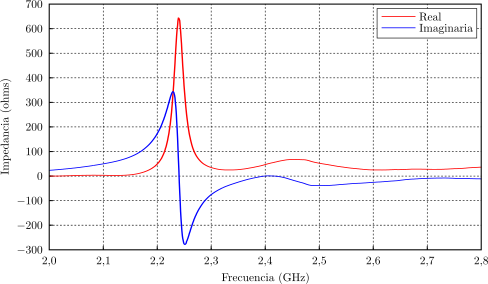
\includegraphics[scale = 1]{Figures/Resultados/resultados_14}
\caption{Medición de la impedancia del alimentador.}
\label{fig_resultados:14}
\end{figure}
%%%%
%%%%
\begin{figure}[H]
\centering
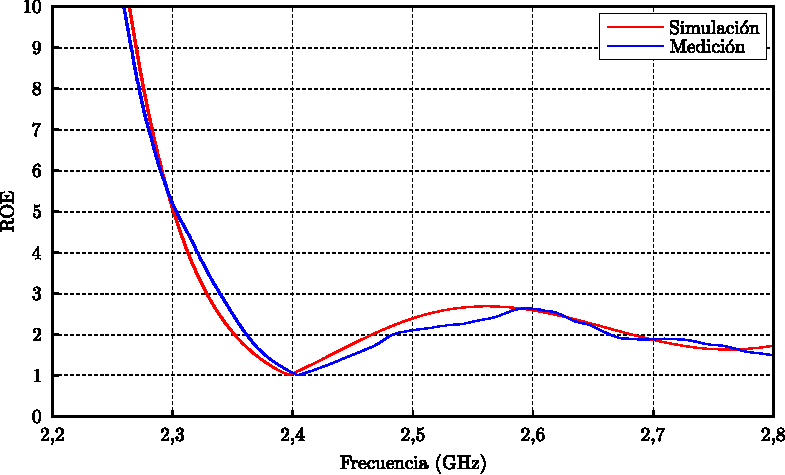
\includegraphics[scale = 1]{Figures/Resultados/resultados_15}
\caption{Simulación y medición de la ROE del alimentador.}
\label{fig_resultados:15}
\end{figure}
%%%%
En la tabla \ref{tabla_mediciones:2} se comparan los valores de impedancia y ROE simulados y medidos del alimentador a la frecuencia de operación, 2,4 GHz. Las incertezas producidas en las mediciones se calcularon en el apéndice \ref{apendice_e}.
%%%%
\begin{table}[H]
\centering
\begin{tabular}{c|c|c|c|}
\cline{2-4}
& \multicolumn{2}{c|}{Impedancia (ohms)} & \multirow{2}{*}{ROE} \\
\cline{2-3}
& Parte real & Parte imaginaria & \\
\hline
\multicolumn{1}{|c|}{Simulación} & 47,72 & 0,75 & 1,05 \\
\hline
\multicolumn{1}{|c|}{Medición} & 47,07 & 0,16 & 1,06 \\
\hline
\end{tabular}
\caption{Comparación entre la simulación y la medición de la impedancia y de la ROE del alimentador.}
\label{tabla_mediciones:2}
\end{table}
%%%%
A partir de los resultados anteriores, se puede observar que los valores obtenidos experimentalmente, tanto para el dimensionamiento del alimentador como para la medición de la impedancia y de la ROE, se aproximan muy bien a los simulados.

Finalmente se ha cortado la guía de onda para que la distancia entre el excitador y el cortocircuito de la guía de onda se ajuste al valor obtenido experimentalmente y se procedió a soldar el cortocircuito definitivo. En la figura \ref{fig_resultados:16} puede observarse el alimentador con el cortocircuito de la guía soldado.
%%%%
\begin{figure}[H]
\centering
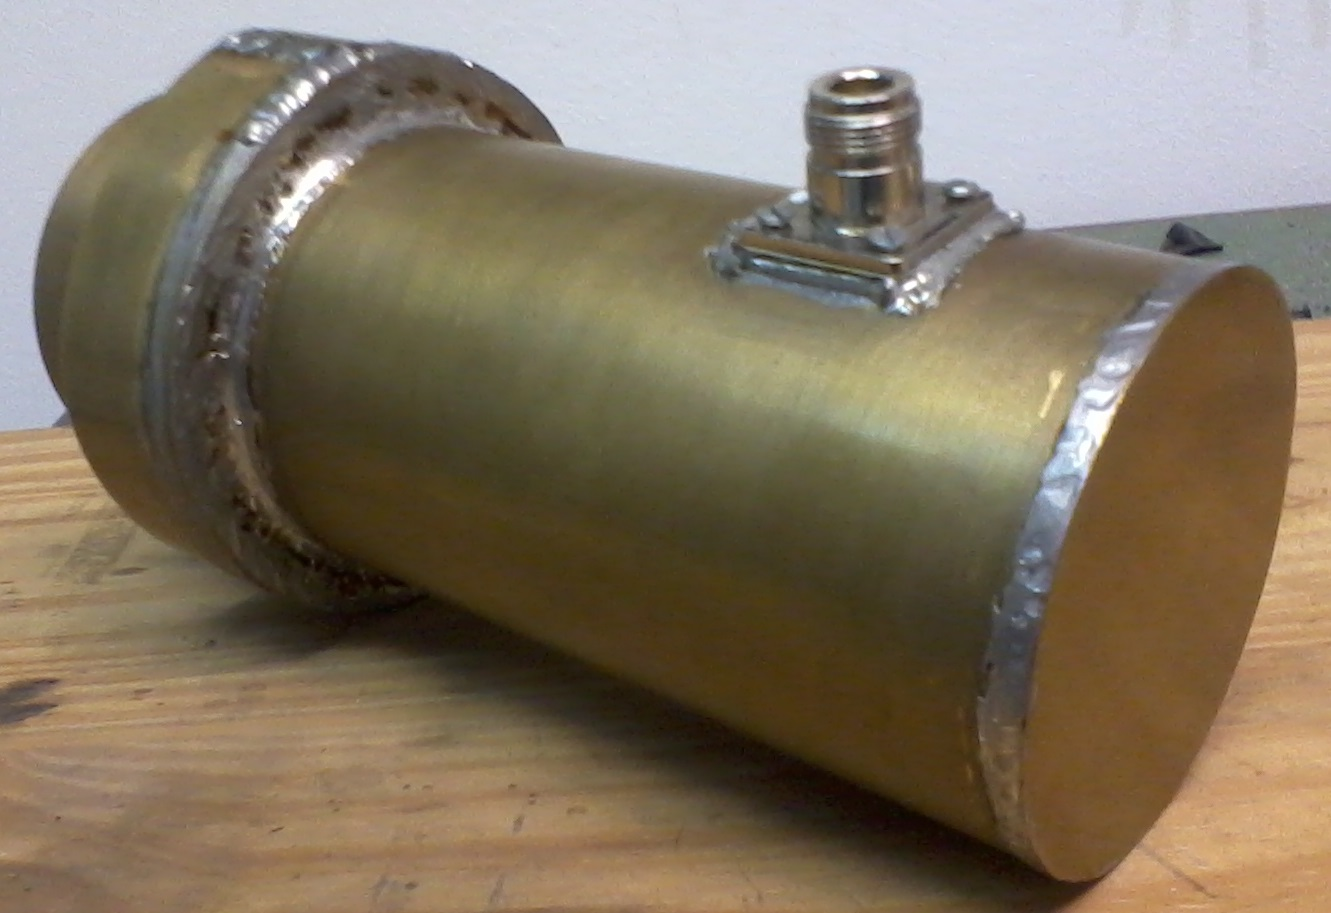
\includegraphics[scale = 0.3]{Figures/Resultados/resultados_16}
\caption{Alimentador con el cortocircuito de la guía soldado.}
\label{fig_resultados:16}
\end{figure}
%%%%

%%%%
\section{Medición del diagrama de radiación}
\label{sec_resultados_med_dia_rad}
%%%%

Para medir el diagrama de radiación del alimentador, se implementó el banco de medición de la figura \ref{fig_resultados:17}.
%%%%
\begin{figure}[H]
\centering
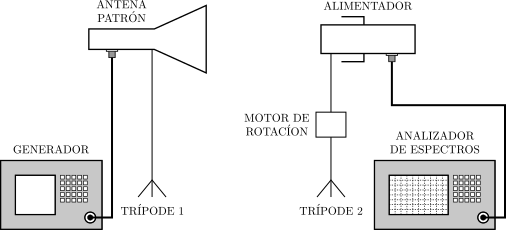
\includegraphics[scale = 1]{Figures/Resultados/resultados_17}
\caption{Banco de medición del diagrama de radiación.}
\label{fig_resultados:17}
\end{figure}
%%%%
Se han medido los planos E y H del diagrama de radiación. Como antena patrón se utilizó una bocina piramidal que, según las simulaciones, tiene una ganancia de aproximadamente 12 dBi. Utilizando esta antena de alta ganancia como patrón y colocando ambas antenas a una altura de 1,8 metros se disminuyen los efectos causados por las reflexiones de las ondas electromagnéticas en el recinto de medición. No se ha medido la ganancia del alimentador porque no se cuenta con la infraestructura necesaria. En la figura \ref{fig_resultados:18} puede observarse la bocina piramidal usada como antena patrón.
%%%%
\begin{figure}[H]
\centering
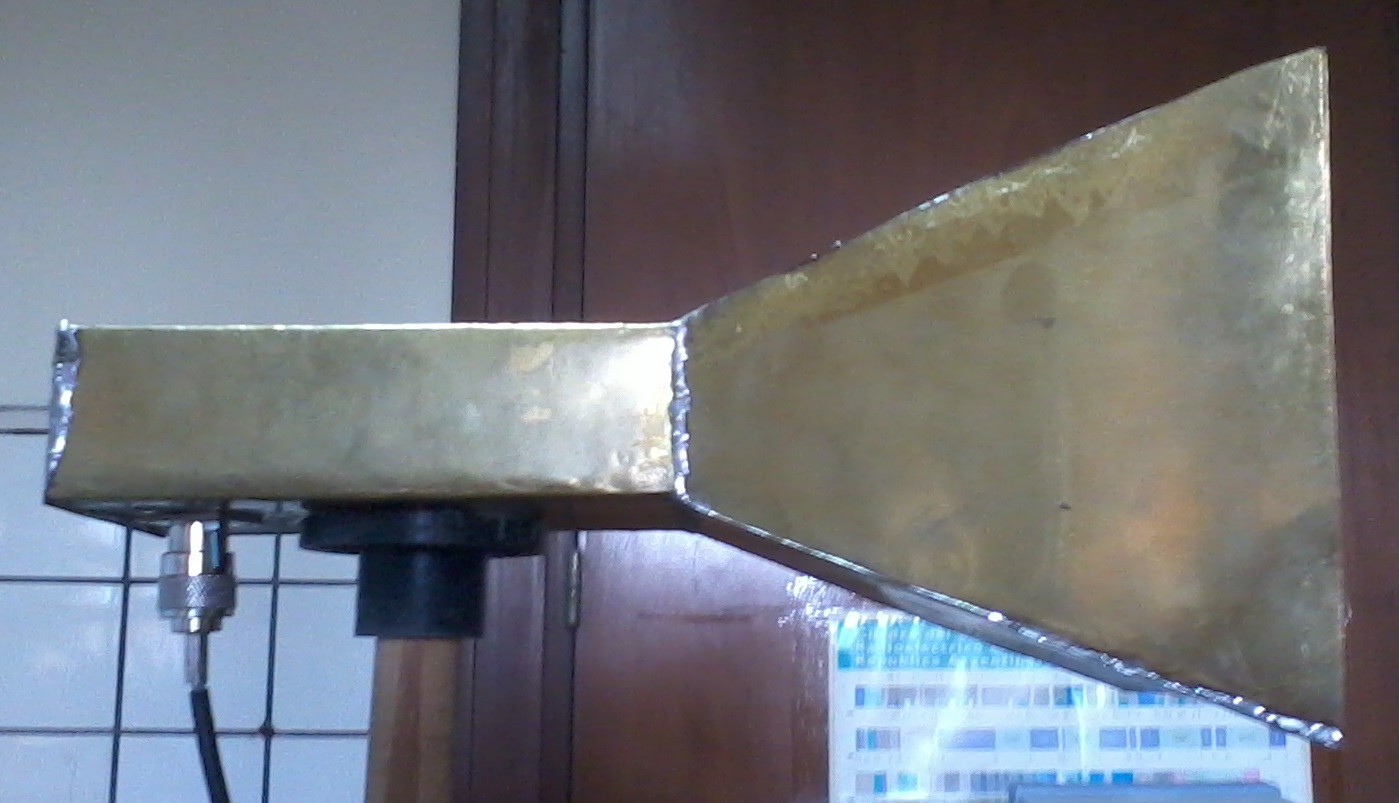
\includegraphics[scale = 0.27]{Figures/Resultados/resultados_18}
\caption{Bocina piramidal empleada como antena patrón.}
\label{fig_resultados:18}
\end{figure}
%%%%
El alimentador se ha instalado sobre un cilindro de madera solidario con el eje de rotación del motor y se ha conectado al analizador de espectros. Para la medición, se ha configurado el analizador de espectros para trabajar con zero span a una frecuencia central de 2,4 GHz. Como el tiempo que el alimentador tarda en dar un giro completo es de aproximadamente 13 segundos, se configuró el barrido del analizador de espectros en 20 segundos para asegurarse que dentro de los valores medidos se tengan dos máximos, que corresponden al instante en que el alimentador esté alineado con la antena patrón.
%%%%
\begin{figure}[H]
\centering
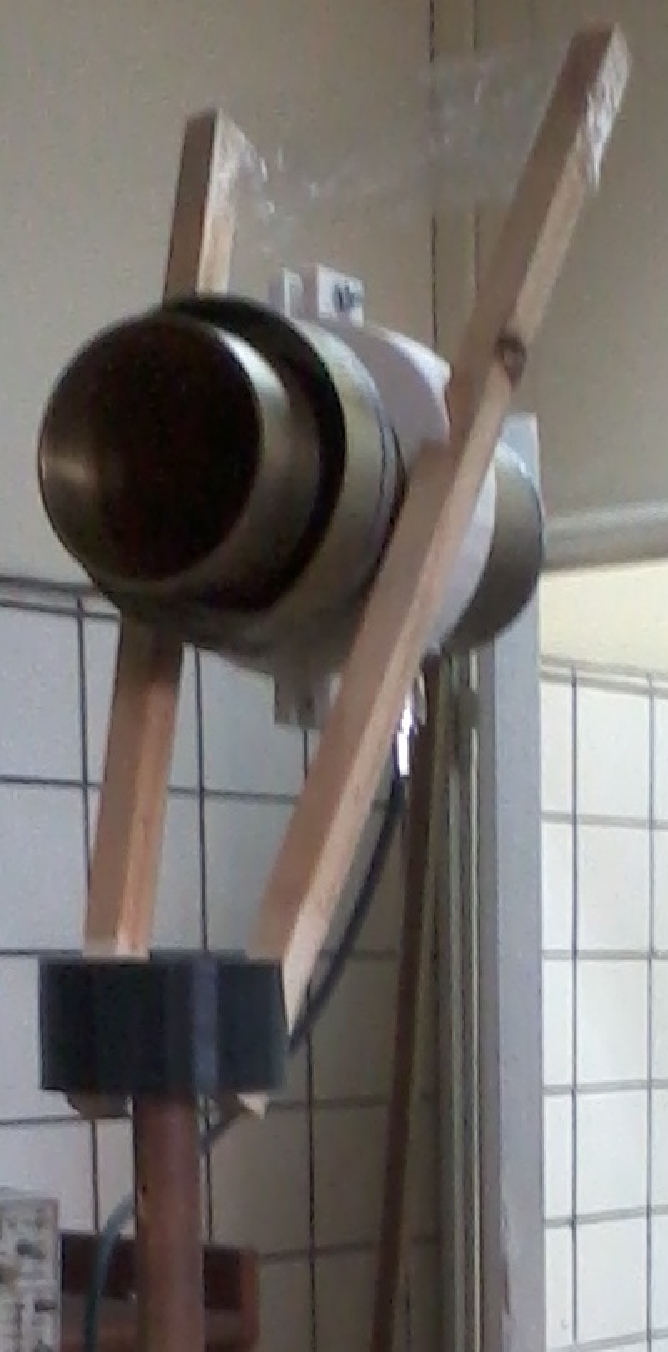
\includegraphics[scale = 0.35]{Figures/Resultados/resultados_19}
\caption{Alimentador instalado sobre el rotador.}
\label{fig_resultados:19}
\end{figure}
%%%%
Para determinar la separación entre la antena patrón y el alimentador, se calculó la distancia de campo lejano; considerando que la máxima dimensión de la antena patrón es de 25 cms, la distancia de campo lejano es:
%%%%
\begin{align*}
D_{cl} = 2\,\dfrac{D^2}{\lambda} = 2\,\dfrac{\left(\text{25 cm}\right)^2}{\text{12,5 cm}} = 1\text{ m}
\end{align*}
%%%%
El banco de medición armado puede observarse en la figura \ref{fig_resultados:20}.
%%%%
\begin{figure}[H]
\centering
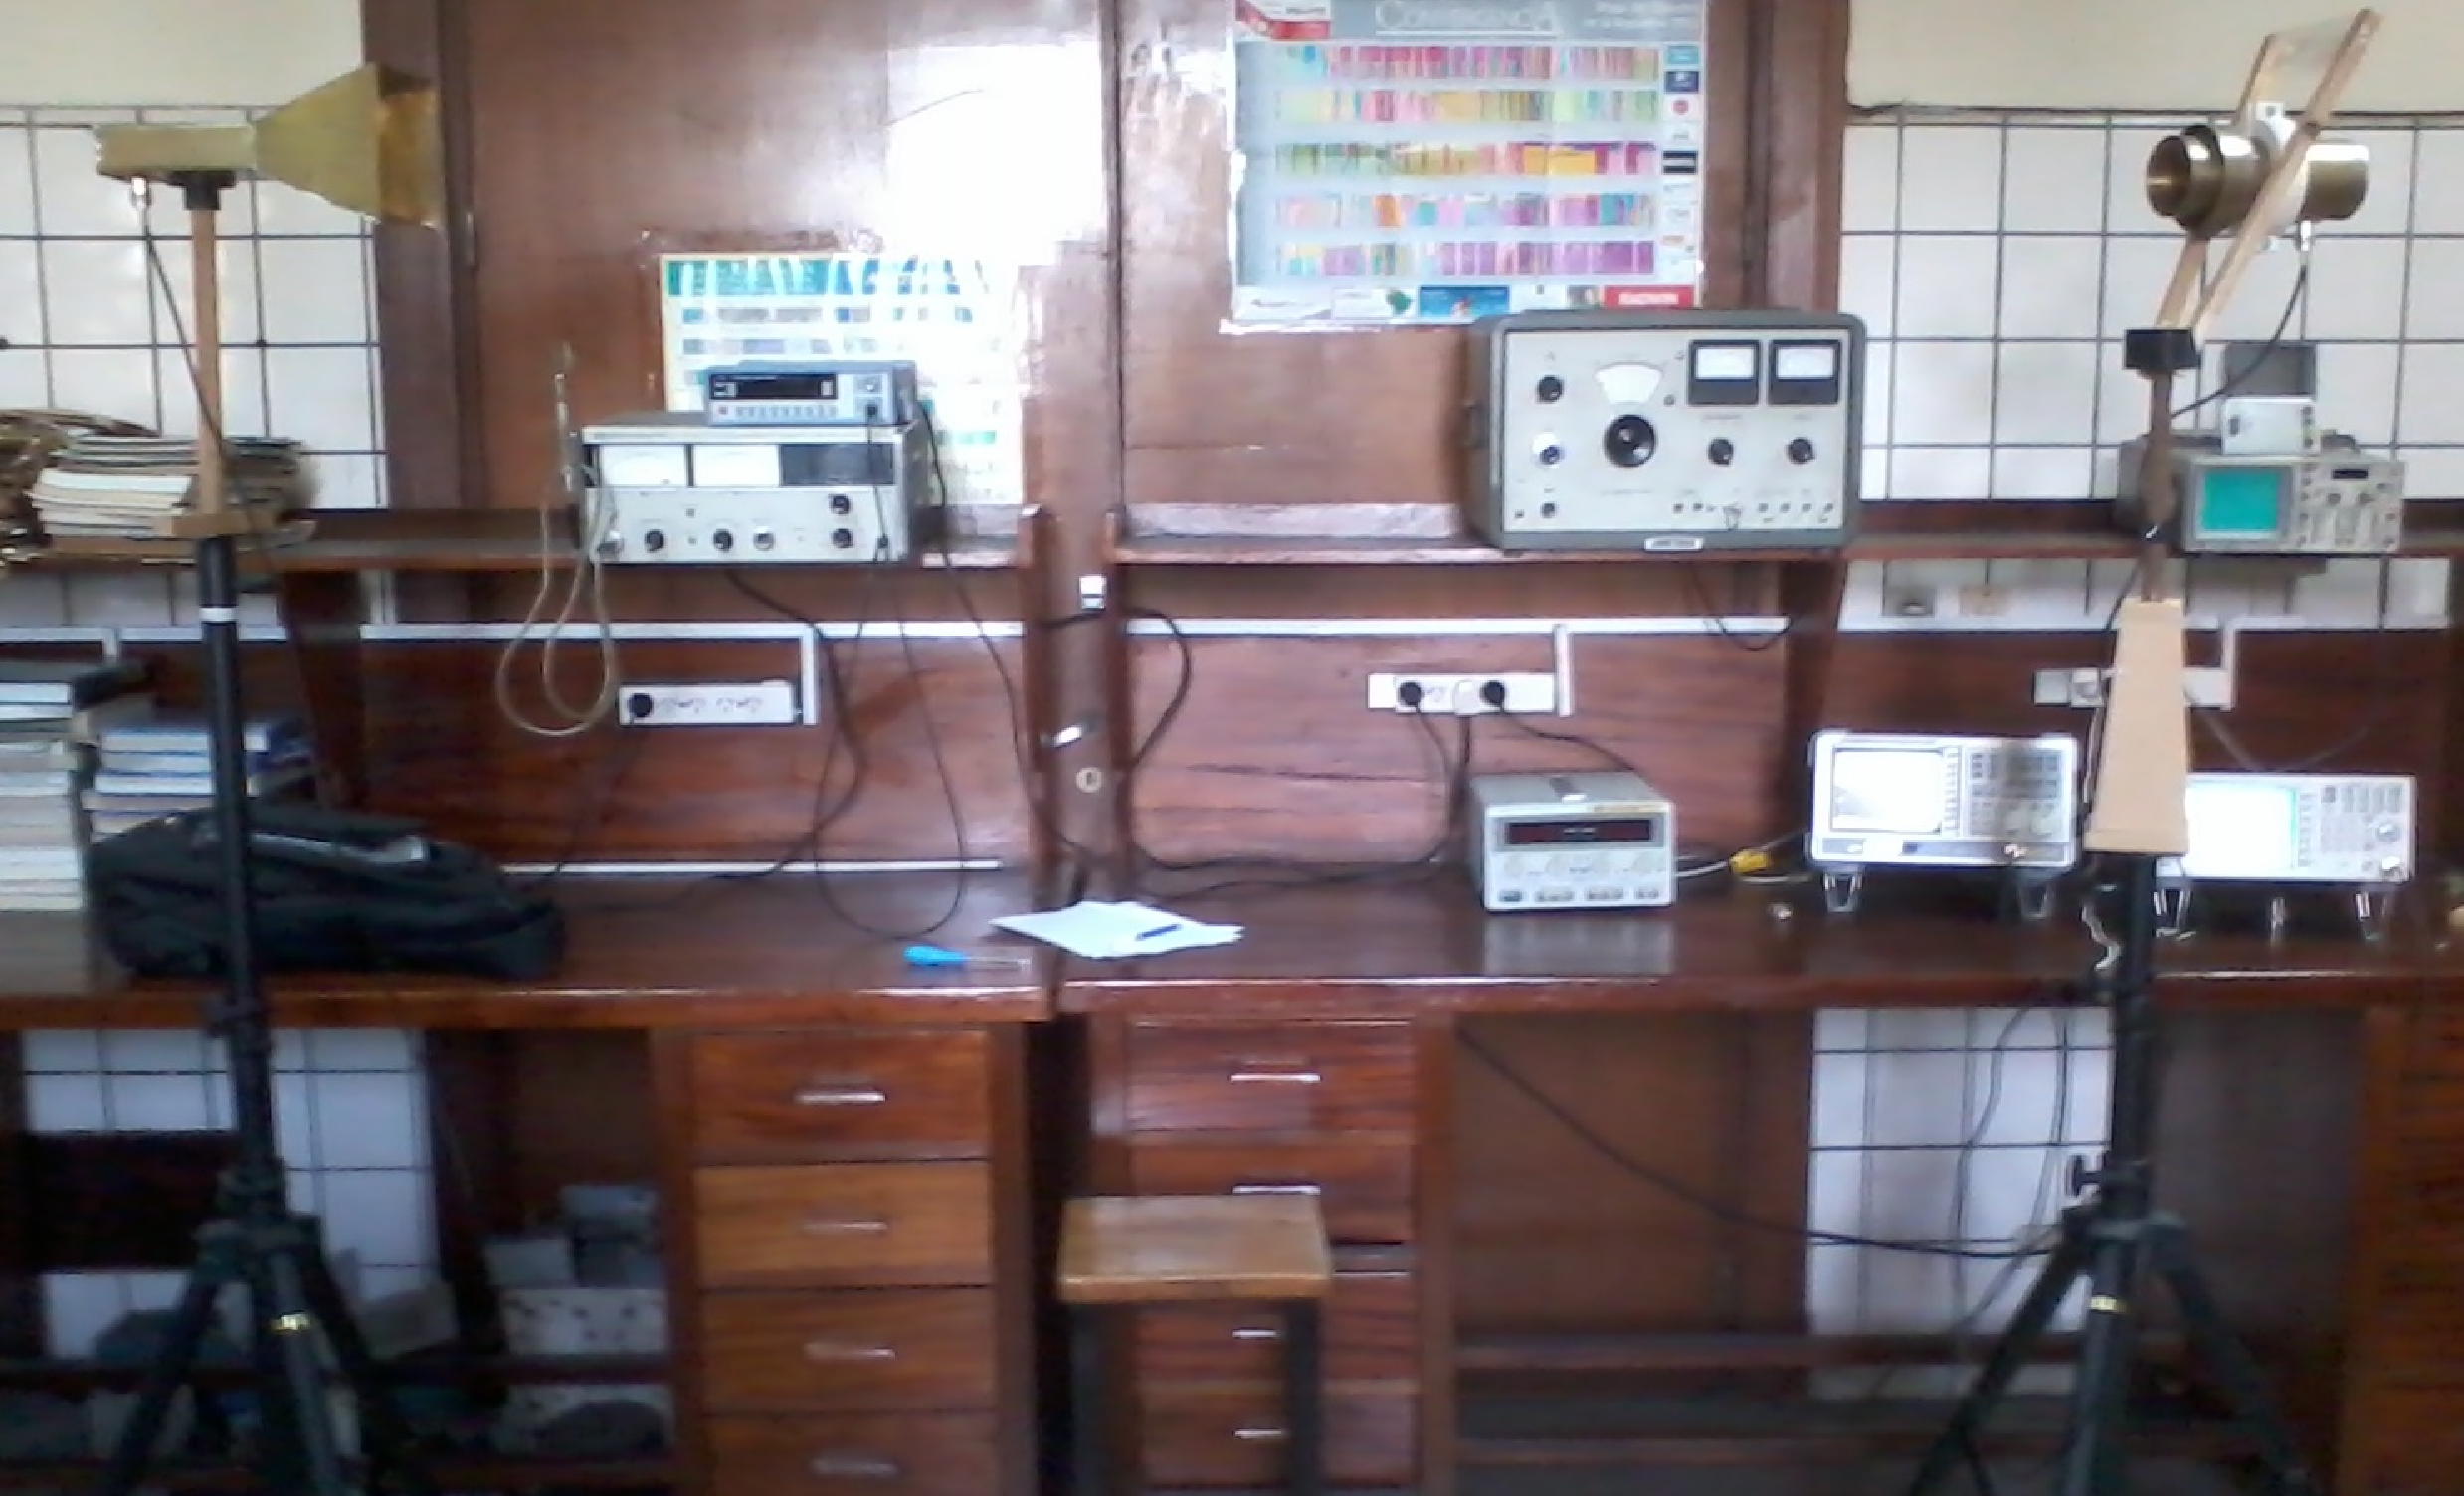
\includegraphics[scale = 0.32]{Figures/Resultados/resultados_20}
\caption{Banco de medición implementado.}
\label{fig_resultados:20}
\end{figure}
%%%%
En las figura \ref{grup_fig_resultados:3} pueden observarse las mediciones de los planos E y H del diagrama de radiación, superpuestos a los diagramas de radiación simulados con el fin de poder contrastar mediciones con simulaciones.
%%%%
\begin{figure} [H]
\centering 
\subfigure[Plano E.]{
\label{fig_resultados:21}
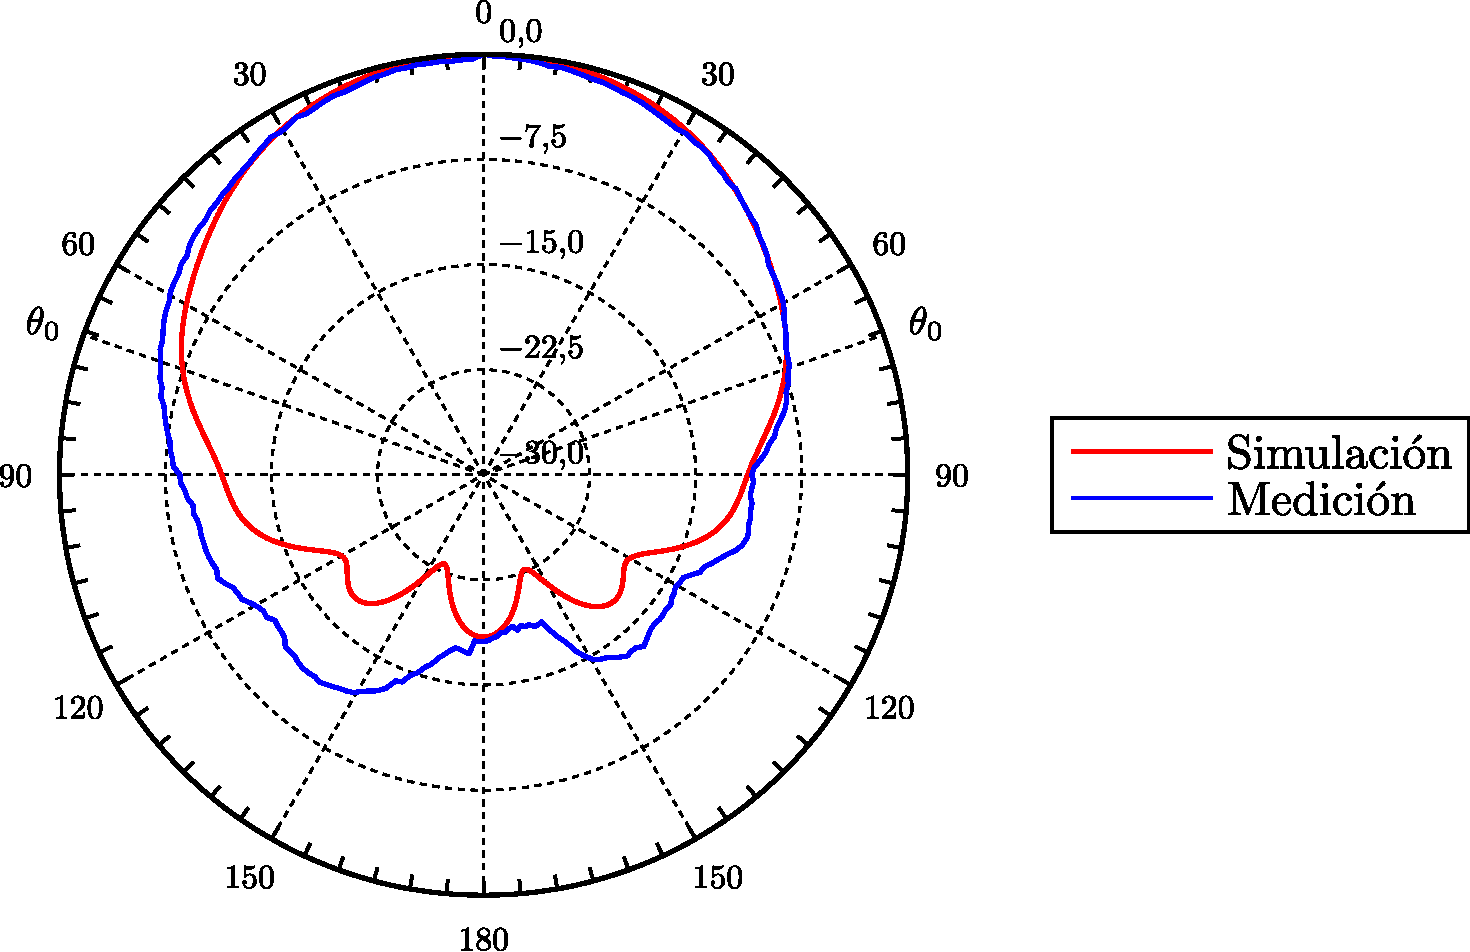
\includegraphics[scale = 0.5]{Figures/Resultados/resultados_21}}
\subfigure[Plano H.]{
\label{fig_resultados:22}
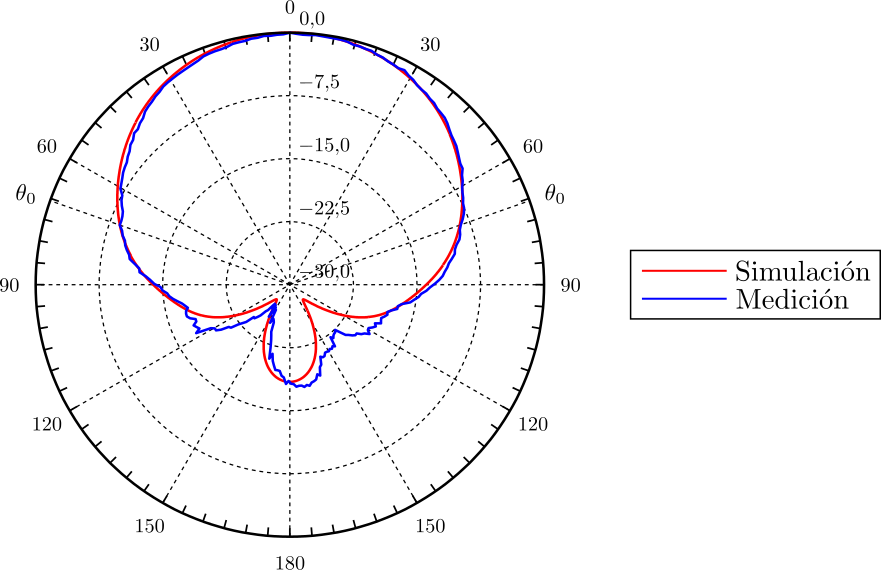
\includegraphics[scale = 0.5]{Figures/Resultados/resultados_22}}
\caption{Simulación y medición de los planos E y H del diagrama de radiación del alimentador.}
\label{grup_fig_resultados:3}
\end{figure}
%%%%
Puede notarse que el Plano E del diagrama de radiación medido presenta una asimetría, que se debe a que en el plano en el que se rota el alimentador para realizar la medición se ubica el conector N y la línea de transmisión coaxial, lo que inevitablemente va a afectar la medición. Sin embargo, puede verse que para valores de $\uptheta$ comprendidos entre 0$^{\circ}$ y 90$^{\circ}$ la medición es coincidente con la simulación.

Para la medición del Plano H, dado que el conector N no se ubica en el plano de rotación del alimentador, la condición de simetría es bien marcada, lo que se evidencia en la medición obtenida, que además de ser muy simétrica, es casi coincidente con la simulación.

En la tabla \ref{tabla_mediciones:3} se compara el ancho de haz principal, la ganancia normalizada en el ángulo $\theta_0$ y la relación frente-espalda obtenidos mediante la simulación y la medición. Las incertezas producidas en las mediciones se calcularon en el apéndice \ref{apendice_e}.
%%%%
\begin{table}[H]
\centering
\begin{tabular}{c|c|c|cc|c|}
\cline{2-6}
& \multicolumn{2}{c|}{Ancho de haz} & \multicolumn{2}{c|}{\multirow{2}{*}{$G_{fn}\left(\theta_0\right)\,$(dB)}} & \multirow{2}{*}{Relación frente}\\
& \multicolumn{2}{c|}{principal (grados)} & & & \multirow{2}{*}{espalda (dB)}\\
\cline{2-5}
& Plano E & Plano H & \multicolumn{1}{|c|}{Plano E} & Plano H &\\
\hline
\multicolumn{1}{|c|}{Simulación} & 82,90 & 81,02 & \multicolumn{1}{|c|}{-7,35} & -8,75 & 18,44\\
\hline
\multicolumn{1}{|c|}{Medición} & 82,37 & 85,22 & \multicolumn{1}{|c|}{-7,33} & -8,91 & 17,71\\
\hline
\end{tabular}
\caption{Comparación entre la simulación y la medición del ancho de haz principal, la ganancia normalizada en el ángulo $\theta_0$ y la relación frente-espalda.}
\label{tabla_mediciones:3}
\end{table}
%%%%
Puede observarse que los valores obtenidos experimentalmente son similares a los simulados.


%%%%
\section{Cálculo de las pérdidas óhmicas del alimentador}
\label{sec_resultados_per_ohm_ali}
%%%%

Las pérdidas óhmicas del alimentador dependen tanto de la conductividad del material conductor con el que se construye la antena como de la frecuencia de operación y de las dimensiones de la guía de onda cilíndrica.

Para una guía de onda cilíndrica y considerando el modo de propagación dominante, las pérdidas por unidad de longitud \cite{Balaniselectro} están dadas por:
%%%%
\begin{align*}
\alpha = \dfrac{R_s}{a\eta_0\sqrt{1 - \left(\dfrac{f_c}{f}\right)^2}}\left[\!\left(\dfrac{f_c}{f}\right)^2 \!+ \dfrac{1}{{\chi '_{11}}^2  - 1}\right]\dfrac{\text{Np}}{\text{m}}
\end{align*}
%%%%
donde:
%%%%
\begin{align*}
Rs = \sqrt{\dfrac{\omega\mu}{2\sigma}} =\text{Resistencia superficial.}
\end{align*}
%%%%
Para el diámetro del alimentador, la frecuencia de corte es:
%%%%
\begin{align*}
f_c = \dfrac{c}{2\pi}\dfrac{\chi '_{11}}{a} = \text{2,22 GHz}
\end{align*}
%%%%
y las pérdidas por unidad de longitud:
%%%%
\begin{align*}
\alpha = \text{0,00543}\,\dfrac{\text{Np}}{\text{m}}
\end{align*}
%%%%
Considerando la longitud de la guía de onda y que 1 Np = 8,6858 dB, la atenuación producida en el alimentador resulta:
%%%%
\begin{align*}
AT \simeq \text{0,01 dB}
\end{align*}
%%%%
La atenuación producida es extremadamente baja, por lo que puede considerarse que la ganancia y la directividad del alimentador son iguales.

%%%%
\section{Simulaciones de polarización cruzada}
\label{sec_resultados_sim_pol_cru}
%%%%

En la sección \ref{sec_polarizacion_cruzada} se ha deducido que la máxima polarización cruzada se produce para el plano $\upphi = 45^{\circ}$, por lo que las simulaciones de polarización cruzada se realizaron solamente para ese plano.

En la figura \ref{fig_resultados:23} se observa la simulación de la copolarización y de la polarización cruzada del alimentador.
%%%%
\begin{figure}[H]
\centering
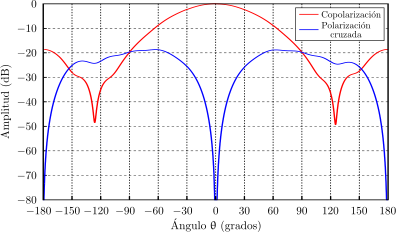
\includegraphics[scale = 1]{Figures/Resultados/resultados_23}
\caption{Simulación de la copolarización y de la polarización cruzada del alimentador para el plano $\upphi = 45^{\circ}$.}
\label{fig_resultados:23}
\end{figure}
%%%%
La relación de polarización cruzada $\rho_L$, cuya expresión es \eqref{ec_intro:78}, según la simulación resulta  $\rho_L$ = 18,63 dB.

En la figura \ref{fig_resultados:24} se observa la simulación de la copolarización y de la polarización cruzada del conjunto formado por el alimentador y el reflector parabólico.
%%%%
\begin{figure}[H]
\centering
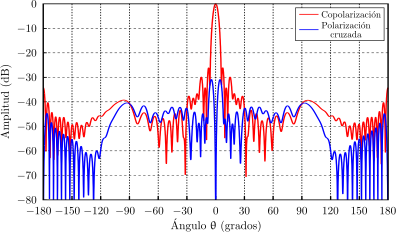
\includegraphics[scale = 1]{Figures/Resultados/resultados_24}
\caption{Simulación de la copolarización y de la polarización cruzada del alimentador con el reflector parabólico para el plano $\upphi = 45^{\circ}$.}
\label{fig_resultados:24}
\end{figure}
%%%%
En la figura \ref{fig_resultados:25} puede observarse la simulación de la copolarización y de la polarización cruzada del conjunto formado por el alimentador y el reflector parabólico para valores de $\uptheta$ menores a 15$^{\circ}$, con el fin de observar detalladamente que sucede en la región cercana a la dirección de propagación principal.
%%%%
\begin{figure}[H]
\centering
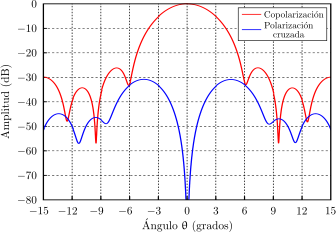
\includegraphics[scale = 1]{Figures/Resultados/resultados_25}
\caption{Simulación de la copolarización y de la polarización cruzada del alimentador con el reflector parabólico para el plano $\upphi = 45^{\circ}$ (detallada).}
\label{fig_resultados:25}
\end{figure}
%%%%
La relación de polarización cruzada, según la simulación, es 30,85 dB, lo que puede considerarse un resultado muy satisfactorio.

%%%%
\section{Simulaciones de diagramas de radiación}
\label{sec_resultados_sim_dia_rad}
%%%%

En la figura \ref{grup_fig_resultados:4} pueden observarse las simulaciones de los planos E y H del diagrama de radiación del conjunto formado por el alimentador y el reflector parabólico.
%%%%
\begin{figure} [H]
\centering 
\subfigure[Plano E.]{
\label{fig_resultados:26}

\includegraphics[scale = 1]{Figures/Resultados/resultados_26}}
\hspace{5mm}
\subfigure[Plano H.]{
\label{fig_resultados:27}

\includegraphics[scale = 1]{Figures/Resultados/resultados_27}}
\caption{Simulación de los planos E y H del diagrama de radiación del alimentador con el reflector parabólico.}
\label{grup_fig_resultados:4}
\end{figure}
%%%%
La directividad máxima y la eficiencia de abertura determinados a partir de la simulación son:
%%%%
\begin{itemize}
\item Directividad $D_0$: 31,68 dBi.
\item Eficiencia de abertura: 71,93 \%.
\end{itemize}
%%%%
En la tabla \ref{tabla_mediciones:4} se muestra el ancho de haz principal y además el ángulo y la amplitud normalizada del primer lóbulo secundario, según la simulación, en los planos E y H.
%%%%
\begin{table}[H]
\centering
\begin{tabular}{c|c|c|c|}
\cline{2-4}
& Ancho de haz & Ángulo 1.$^{\text{er}}$ lóbulo & Amplitud normalizada 1.$^{\text{er}}$ \\
& principal (grados) & secundario (grados) & lóbulo secundario (dB) \\
\hline
\multicolumn{1}{|c|}{Plano E} & 4,68 & 7,17 & -25,77 \\
\hline
\multicolumn{1}{|c|}{Plano H} & 4,68 & 7,45 & -25,87 \\
\hline
\end{tabular}
\caption{Valores obtenidos por simulación del ancho de haz principal y del ángulo y la amplitud del primer lóbulo secundario en los planos E y H del diagrama de radiación.}
\label{tabla_mediciones:4}
\end{table}
%%%%
Viendo los resultados, tener una eficiencia de abertura superior al 70 \% es un muy buen resultado. Sin embargo, en la práctica existen otros factores que inciden en la eficiencia además de la iluminación del reflector, como las irregularidades en la superficie y la geometría del reflector y los desplazamientos axiales y radiales del alimentador respecto al foco.

Finalmente, en las figuras \ref{fig_resultados:28} y \ref{fig_resultados:29} se observan los diagramas de radiación 3D del alimentador y del alimentador con el reflector parabólico respectivamente.

%%%%
\begin{figure}[H]
\centering
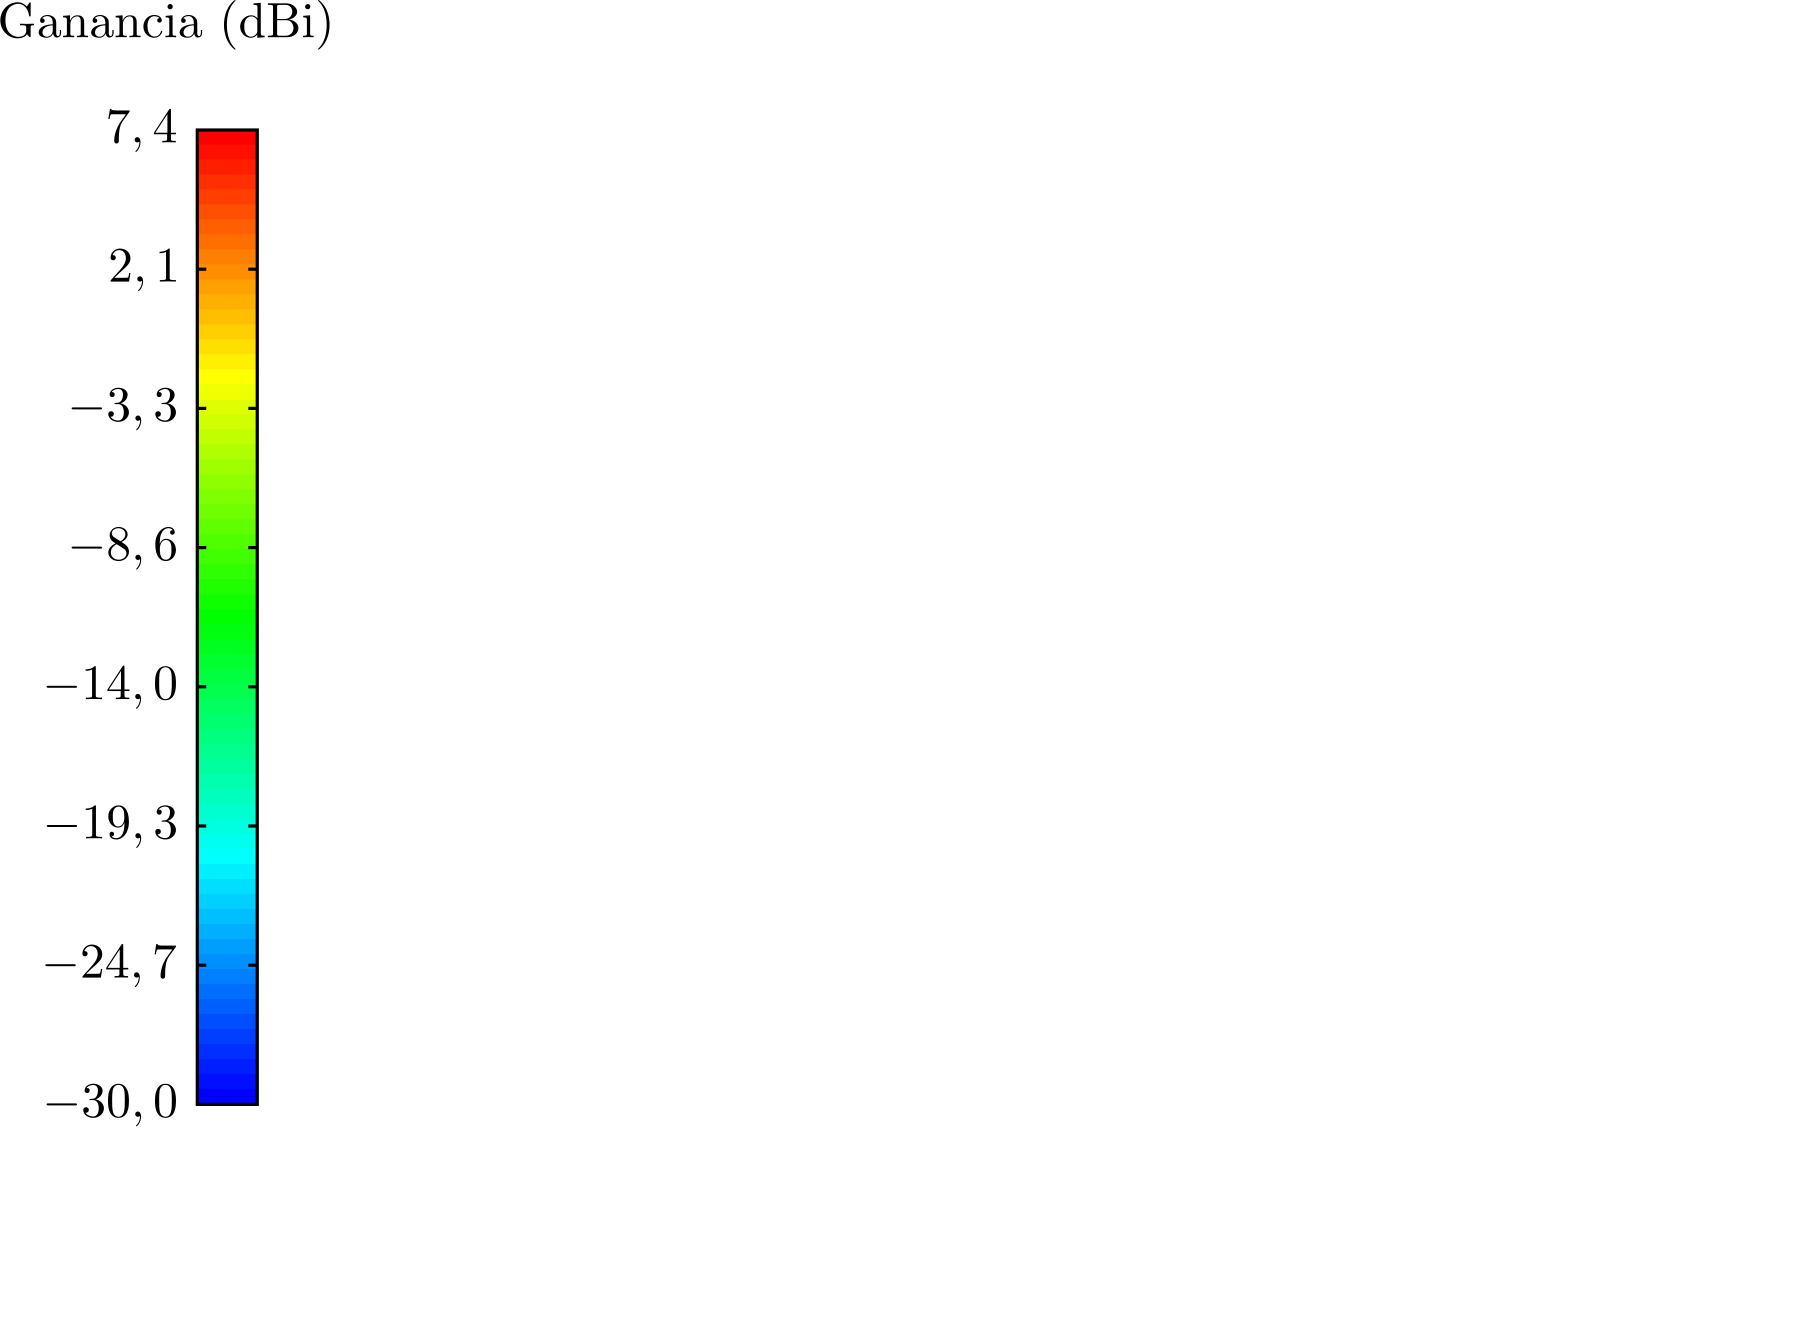
\includegraphics[scale = 0.25]{Figures/Resultados/resultados_28}
\caption{Simulación del diagrama de radiación 3D del alimentador.}
\label{fig_resultados:28}
\end{figure}
%%%%
%%%%
\begin{figure}[H]
\centering
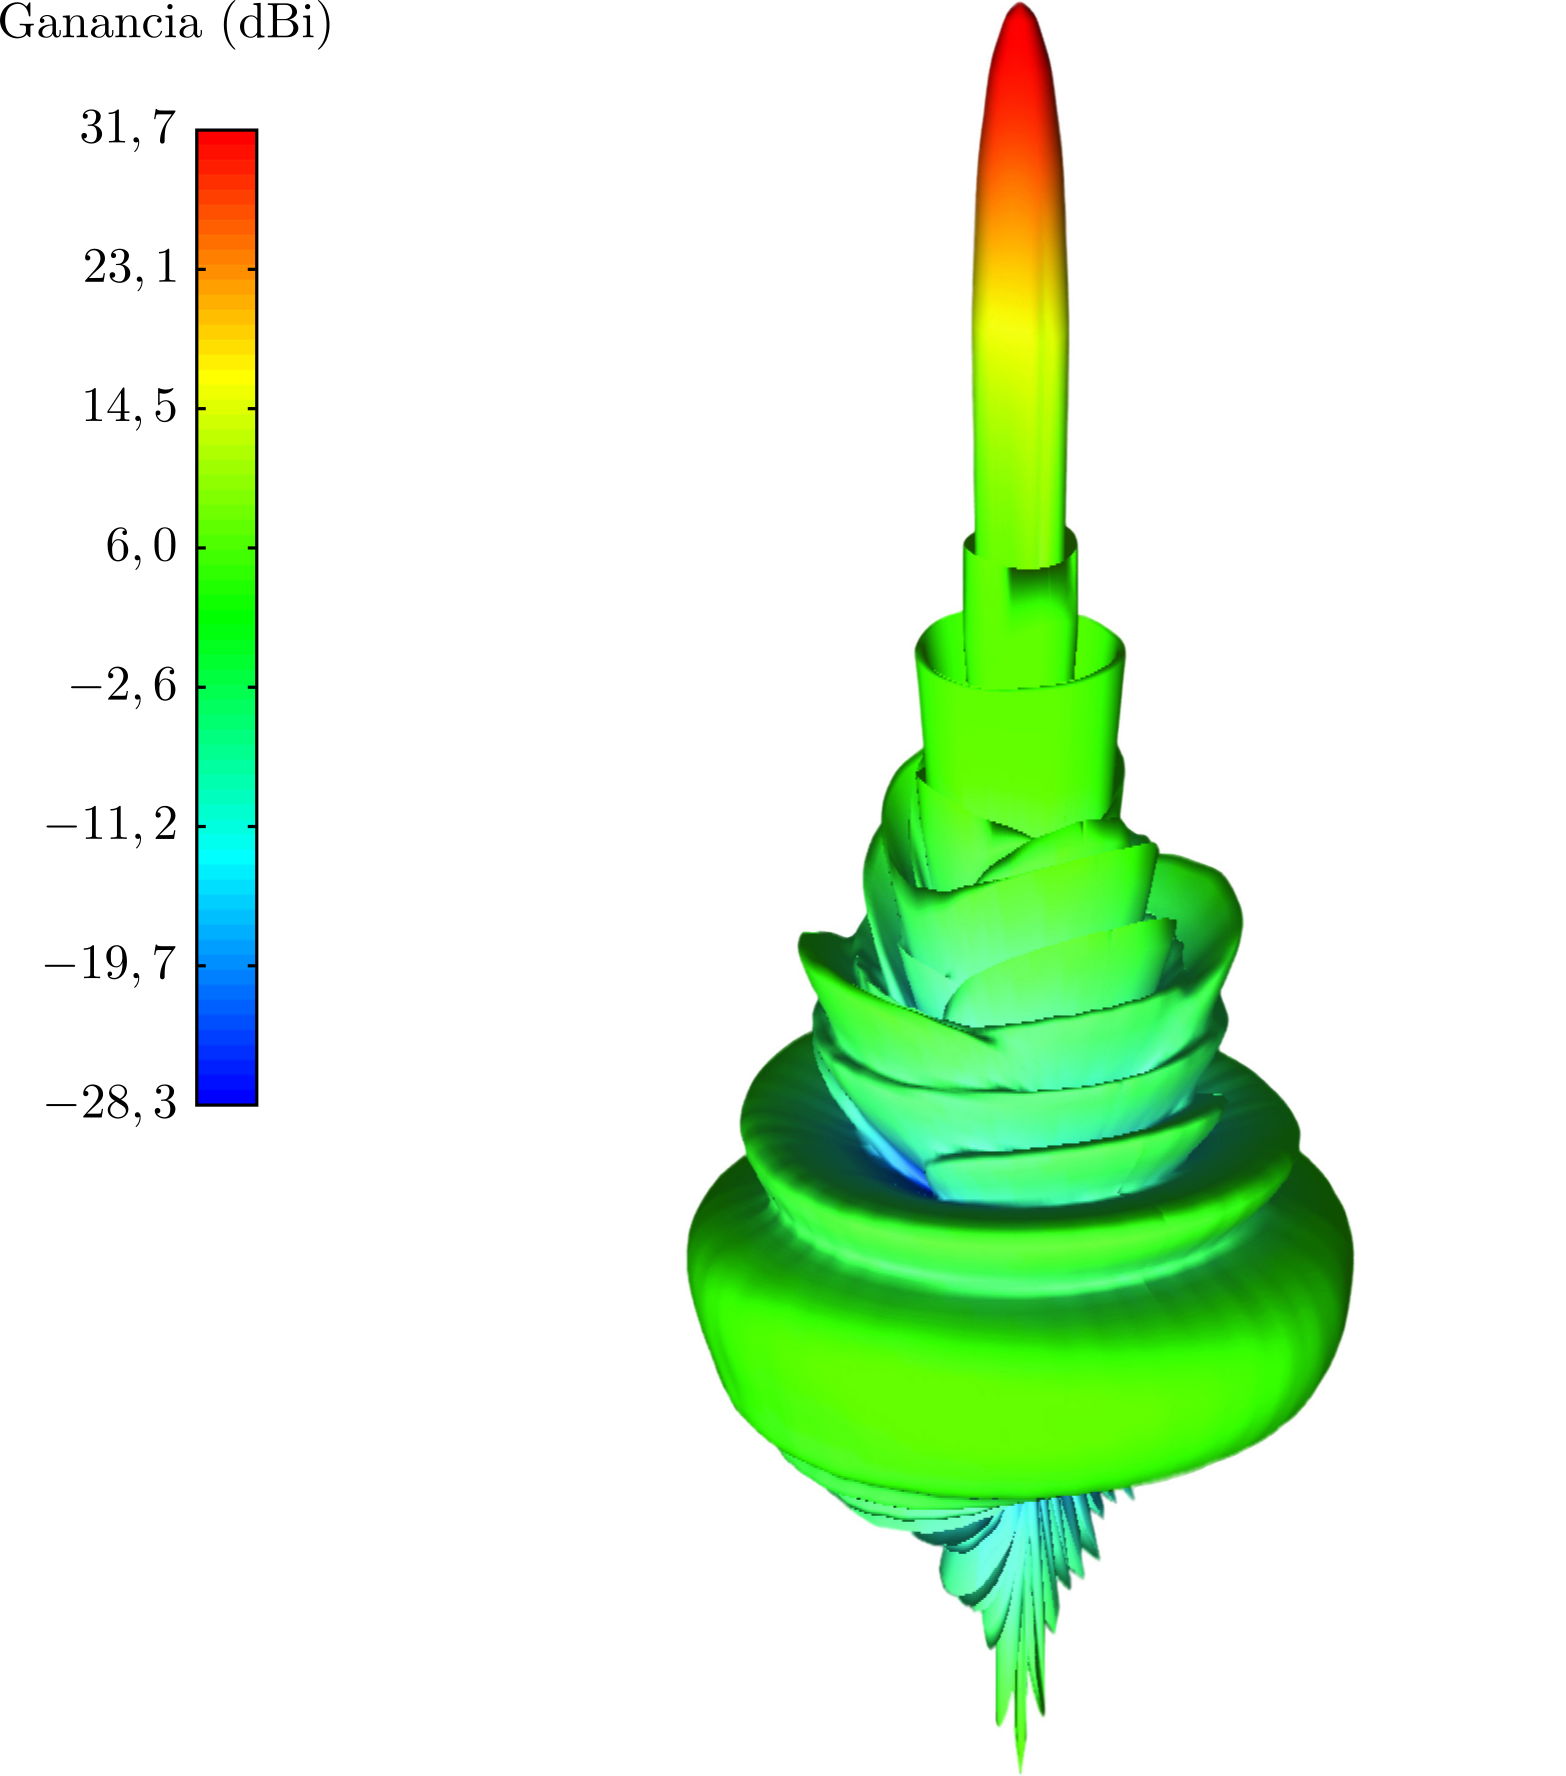
\includegraphics[scale = 0.25]{Figures/Resultados/resultados_29}
\caption{Simulación del diagrama de radiación 3D del alimentador con el reflector parabólico.}
\label{fig_resultados:29}
\end{figure}
%%%%